\documentclass[a4paper]{book}
\usepackage{makeidx}
\usepackage{natbib}
\usepackage{graphicx}
\usepackage{multicol}
\usepackage{float}
\usepackage{listings}
\usepackage{color}
\usepackage{ifthen}
\usepackage[table]{xcolor}
\usepackage{textcomp}
\usepackage{alltt}
\usepackage{ifpdf}
\ifpdf
\usepackage[pdftex,
            pagebackref=true,
            colorlinks=true,
            linkcolor=blue,
            unicode
           ]{hyperref}
\else
\usepackage[ps2pdf,
            pagebackref=true,
            colorlinks=true,
            linkcolor=blue,
            unicode
           ]{hyperref}
\usepackage{pspicture}
\fi
\usepackage[utf8]{inputenc}
\usepackage{mathptmx}
\usepackage[scaled=.90]{helvet}
\usepackage{courier}
\usepackage{sectsty}
\usepackage[titles]{tocloft}
\usepackage{doxygen}
\lstset{language=C++,inputencoding=utf8,basicstyle=\footnotesize,breaklines=true,breakatwhitespace=true,tabsize=8,numbers=left }
\makeindex
\setcounter{tocdepth}{3}
\renewcommand{\footrulewidth}{0.4pt}
\renewcommand{\familydefault}{\sfdefault}
\hfuzz=15pt
\setlength{\emergencystretch}{15pt}
\hbadness=750
\tolerance=750
\begin{document}
\hypersetup{pageanchor=false,citecolor=blue}
\begin{titlepage}
\vspace*{7cm}
\begin{center}
{\Large \-D\-D2.5\-D \\[1ex]\large 0 }\\
\vspace*{1cm}
{\large \-Generated by Doxygen 1.7.6.1}\\
\vspace*{0.5cm}
{\small Mon Apr 22 2013 11:33:35}\\
\end{center}
\end{titlepage}
\clearemptydoublepage
\pagenumbering{roman}
\tableofcontents
\clearemptydoublepage
\pagenumbering{arabic}
\hypersetup{pageanchor=true,citecolor=blue}
\chapter{\-Data \-Structure \-Index}
\section{\-Class \-Hierarchy}
\-This inheritance list is sorted roughly, but not completely, alphabetically\-:\begin{DoxyCompactList}
\item \contentsline{section}{\-Defect}{\pageref{d5/d4f/classDefect}}{}
\item \contentsline{section}{\-Matrix33}{\pageref{de/d82/classMatrix33}}{}
\begin{DoxyCompactList}
\item \contentsline{section}{\-Rotation\-Matrix}{\pageref{d2/d4a/classRotationMatrix}}{}
\item \contentsline{section}{\-Strain}{\pageref{d1/d3c/classStrain}}{}
\item \contentsline{section}{\-Stress}{\pageref{d1/d1c/classStress}}{}
\end{DoxyCompactList}
\item \contentsline{section}{\-Vector3d}{\pageref{df/dd0/classVector3d}}{}
\end{DoxyCompactList}

\chapter{\-Data \-Structure \-Index}
\section{\-Data \-Structures}
\-Here are the data structures with brief descriptions\-:\begin{DoxyCompactList}
\item\contentsline{section}{\hyperlink{classDefect}{\-Defect} }{\pageref{d5/d4f/classDefect}}{}
\item\contentsline{section}{\hyperlink{classMatrix33}{\-Matrix33} }{\pageref{de/d82/classMatrix33}}{}
\item\contentsline{section}{\hyperlink{classVector3d}{\-Vector3d} }{\pageref{df/dd0/classVector3d}}{}
\end{DoxyCompactList}

\chapter{\-File \-Index}
\section{\-File \-List}
\-Here is a list of all files with brief descriptions\-:\begin{DoxyCompactList}
\item\contentsline{section}{\hyperlink{constants_8h}{constants.\-h} \\*\-Definition of constants used in the program }{\pageref{d2/d6f/constants_8h}}{}
\item\contentsline{section}{\hyperlink{defect_8cpp}{defect.\-cpp} \\*\-Definition of member functions of the \hyperlink{classDefect}{\-Defect} class }{\pageref{dd/def/defect_8cpp}}{}
\item\contentsline{section}{\hyperlink{defect_8h}{defect.\-h} \\*\-Definition of the \hyperlink{classDefect}{\-Defect} class }{\pageref{df/d55/defect_8h}}{}
\item\contentsline{section}{\hyperlink{dislocation_8cpp}{dislocation.\-cpp} \\*\-Definition of constructors and member functions of the \hyperlink{classDislocation}{\-Dislocation} class }{\pageref{d3/d7f/dislocation_8cpp}}{}
\item\contentsline{section}{\hyperlink{dislocation_8h}{dislocation.\-h} \\*\-Definition of the \hyperlink{classDislocation}{\-Dislocation} class }{\pageref{de/df3/dislocation_8h}}{}
\item\contentsline{section}{\hyperlink{dislocationDefaults_8h}{dislocation\-Defaults.\-h} \\*\-Definition of certain default values for members of the \hyperlink{classDislocation}{\-Dislocation} class }{\pageref{d4/da6/dislocationDefaults_8h}}{}
\item\contentsline{section}{\hyperlink{dislocationSource_8cpp}{dislocation\-Source.\-cpp} \\*\-Definition of the member functions of the \hyperlink{classDislocationSource}{\-Dislocation\-Source} class }{\pageref{d8/d5c/dislocationSource_8cpp}}{}
\item\contentsline{section}{\hyperlink{dislocationSource_8h}{dislocation\-Source.\-h} \\*\-Definition of the \hyperlink{classDislocationSource}{\-Dislocation\-Source} class }{\pageref{da/d0c/dislocationSource_8h}}{}
\item\contentsline{section}{\hyperlink{dislocationSourceDefaults_8h}{dislocation\-Source\-Defaults.\-h} \\*\-Definition of certain default values for members of the \hyperlink{classDislocationSource}{\-Dislocation\-Source} class }{\pageref{d4/d0f/dislocationSourceDefaults_8h}}{}
\item\contentsline{section}{\hyperlink{matrix33_8cpp}{matrix33.\-cpp} \\*\-Definition of the member functions and operators of the \hyperlink{classMatrix33}{\-Matrix33} class }{\pageref{d8/d8e/matrix33_8cpp}}{}
\item\contentsline{section}{\hyperlink{matrix33_8h}{matrix33.\-h} \\*\-Definition of the \hyperlink{classMatrix33}{\-Matrix33} class }{\pageref{db/d46/matrix33_8h}}{}
\item\contentsline{section}{\hyperlink{parameter_8cpp}{parameter.\-cpp} \\*\-Definition of member functions of the \hyperlink{classParameter}{\-Parameter} class which will hold all simulation parameters }{\pageref{d4/d98/parameter_8cpp}}{}
\item\contentsline{section}{\hyperlink{parameter_8h}{parameter.\-h} \\*\-Declaration of the \hyperlink{classParameter}{\-Parameter} class which will hold all simulation parameters }{\pageref{d2/d2a/parameter_8h}}{}
\item\contentsline{section}{\hyperlink{rotationMatrix_8cpp}{rotation\-Matrix.\-cpp} \\*\-Definition of the \hyperlink{classRotationMatrix}{\-Rotation\-Matrix} class member functions }{\pageref{d9/d5c/rotationMatrix_8cpp}}{}
\item\contentsline{section}{\hyperlink{rotationMatrix_8h}{rotation\-Matrix.\-h} \\*\-Definition of the \hyperlink{classRotationMatrix}{\-Rotation\-Matrix} class }{\pageref{da/d76/rotationMatrix_8h}}{}
\item\contentsline{section}{\hyperlink{simulateSingleSlipPlane_8cpp}{simulate\-Single\-Slip\-Plane.\-cpp} \\*\-Defintion various functions to simulate dislocation motion on a single slip plane }{\pageref{d5/d1f/simulateSingleSlipPlane_8cpp}}{}
\item\contentsline{section}{\hyperlink{simulateSingleSlipPlane_8h}{simulate\-Single\-Slip\-Plane.\-h} \\*\-Declaration various functions to simulate dislocation motion on a single slip plane }{\pageref{d2/d56/simulateSingleSlipPlane_8h}}{}
\item\contentsline{section}{\hyperlink{slipPlane_8cpp}{slip\-Plane.\-cpp} \\*\-Definition of the member functions of the \hyperlink{classSlipPlane}{\-Slip\-Plane} class }{\pageref{db/dab/slipPlane_8cpp}}{}
\item\contentsline{section}{\hyperlink{slipPlane_8h}{slip\-Plane.\-h} \\*\-Definition of the \hyperlink{classSlipPlane}{\-Slip\-Plane} class }{\pageref{d5/d03/slipPlane_8h}}{}
\item\contentsline{section}{\hyperlink{slipPlaneDefaults_8h}{slip\-Plane\-Defaults.\-h} \\*\-Definition of certain default values for members of the \hyperlink{classSlipPlane}{\-Slip\-Plane} class }{\pageref{d1/d4f/slipPlaneDefaults_8h}}{}
\item\contentsline{section}{\hyperlink{standardSlipSystem_8cpp}{standard\-Slip\-System.\-cpp} \\*\-Definition of the member functions of the \hyperlink{classStandardSlipSystem}{\-Standard\-Slip\-System} class }{\pageref{d8/d92/standardSlipSystem_8cpp}}{}
\item\contentsline{section}{\hyperlink{standardSlipSystem_8h}{standard\-Slip\-System.\-h} \\*\-Definition of the \hyperlink{classStandardSlipSystem}{\-Standard\-Slip\-System} class }{\pageref{d0/ddd/standardSlipSystem_8h}}{}
\item\contentsline{section}{\hyperlink{statistics_8cpp}{statistics.\-cpp} \\*\-Definition of member functions of the \hyperlink{classStatistics}{\-Statistics} class which will hold the flag and frequency for various stastics }{\pageref{d1/d45/statistics_8cpp}}{}
\item\contentsline{section}{\hyperlink{statistics_8h}{statistics.\-h} \\*\-Declaration of the \hyperlink{classStatistics}{\-Statistics} class which will hold the flag and frequency for various stastics }{\pageref{d7/dc5/statistics_8h}}{}
\item\contentsline{section}{\hyperlink{strain_8cpp}{strain.\-cpp} \\*\-Definition of the member functions if the \hyperlink{classStrain}{\-Strain} class }{\pageref{d7/db1/strain_8cpp}}{}
\item\contentsline{section}{\hyperlink{strain_8h}{strain.\-h} \\*\-Definition of the \hyperlink{classStrain}{\-Strain} class }{\pageref{df/dc2/strain_8h}}{}
\item\contentsline{section}{\hyperlink{stress_8cpp}{stress.\-cpp} \\*\-Definition of the member functions if the \hyperlink{classStress}{\-Stress} class }{\pageref{d4/d58/stress_8cpp}}{}
\item\contentsline{section}{\hyperlink{stress_8h}{stress.\-h} \\*\-Definition of the \hyperlink{classStress}{\-Stress} class }{\pageref{d2/d50/stress_8h}}{}
\item\contentsline{section}{\hyperlink{tools_8cpp}{tools.\-cpp} \\*\-Definition various tools }{\pageref{d3/d62/tools_8cpp}}{}
\item\contentsline{section}{\hyperlink{tools_8h}{tools.\-h} \\*\-Declaration various tools }{\pageref{d5/da5/tools_8h}}{}
\item\contentsline{section}{\hyperlink{vector3d_8cpp}{vector3d.\-cpp} \\*\-Definition of member functions and operators of the \hyperlink{classVector3d}{\-Vector3d} class }{\pageref{d7/d35/vector3d_8cpp}}{}
\item\contentsline{section}{\hyperlink{vector3d_8h}{vector3d.\-h} \\*\-Definition of the \hyperlink{classVector3d}{\-Vector3d} class }{\pageref{d9/df8/vector3d_8h}}{}
\end{DoxyCompactList}

\chapter{\-Data \-Structure \-Documentation}
\hypertarget{classDefect}{\section{\-Defect \-Class \-Reference}
\label{d5/d4f/classDefect}\index{\-Defect@{\-Defect}}
}


\-Class \hyperlink{classDefect}{\-Defect} representing a generic defect in a material.  




{\ttfamily \#include $<$defect.\-h$>$}



\-Inheritance diagram for \-Defect\-:\nopagebreak
\begin{figure}[H]
\begin{center}
\leavevmode
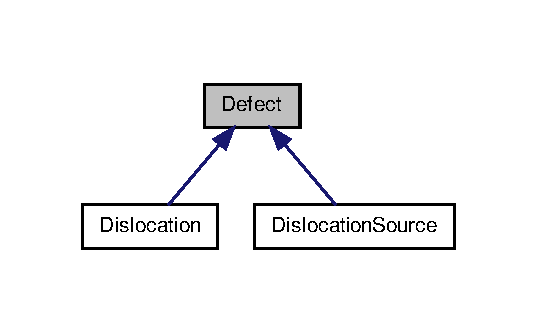
\includegraphics[width=144pt]{de/d48/classDefect__inherit__graph}
\end{center}
\end{figure}


\-Collaboration diagram for \-Defect\-:\nopagebreak
\begin{figure}[H]
\begin{center}
\leavevmode
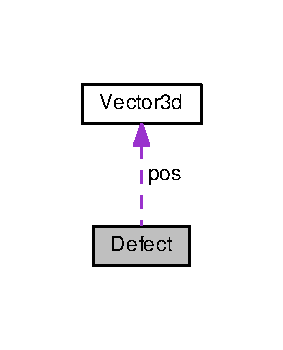
\includegraphics[width=136pt]{d7/d09/classDefect__coll__graph}
\end{center}
\end{figure}
\subsection*{\-Public \-Member \-Functions}
\begin{DoxyCompactItemize}
\item 
\hyperlink{classDefect_afc84dd2d7250a01746ee67b002dbbad9}{\-Defect} ()
\begin{DoxyCompactList}\small\item\em \-Default constructor. \end{DoxyCompactList}\item 
\hyperlink{classDefect_aaddcb1db4b47037adf2e495665f41bab}{\-Defect} (double x, double y, double z)
\begin{DoxyCompactList}\small\item\em \-Constructor specifying the position. \end{DoxyCompactList}\item 
\hyperlink{classDefect_a5bd123214102a5115c46b0a15653d29b}{\-Defect} (double $\ast$p)
\begin{DoxyCompactList}\small\item\em \-Constructor specifying the position. \end{DoxyCompactList}\item 
void \hyperlink{classDefect_a2d233d13a8a93f6fba463a1fbc1c6c9f}{set\-Position} (double $\ast$a)
\begin{DoxyCompactList}\small\item\em \-Sets the position of the defect. \end{DoxyCompactList}\item 
void \hyperlink{classDefect_ad1a6acd8399d2ecabb7ce2b77623bbec}{set\-Position} (double x, double y, double z)
\begin{DoxyCompactList}\small\item\em \-Sets the position of the defect. \end{DoxyCompactList}\item 
void \hyperlink{classDefect_a5a65f73da6a572d9e7109b31239e441d}{set\-X} (double x)
\begin{DoxyCompactList}\small\item\em \-Sets the \-X-\/coordinate of the defect. \end{DoxyCompactList}\item 
void \hyperlink{classDefect_a268606391a4eaee3de029d2005648b6f}{set\-Y} (double y)
\begin{DoxyCompactList}\small\item\em \-Sets the \-Y-\/coordinate of the defect. \end{DoxyCompactList}\item 
void \hyperlink{classDefect_abb0b16c44a1b04d782f5c5f598b49d5b}{set\-Z} (double z)
\begin{DoxyCompactList}\small\item\em \-Sets the \-Z-\/coordinate of the defect. \end{DoxyCompactList}\item 
double $\ast$ \hyperlink{classDefect_a6842fba3ad14032766ccf0437afcbced}{get\-Position} ()
\begin{DoxyCompactList}\small\item\em \-Returns in an array the position. \end{DoxyCompactList}\item 
void \hyperlink{classDefect_aace5c752b85c368631746abc3d5bd714}{get\-Position} (double $\ast$a)
\begin{DoxyCompactList}\small\item\em \-Returns the array position in a pre-\/allocated array. \end{DoxyCompactList}\item 
double \hyperlink{classDefect_a01b96c453c13db82b5835682e1849dc0}{get\-X} ()
\begin{DoxyCompactList}\small\item\em \-Returns the \-X-\/coordinate of the defect. \end{DoxyCompactList}\item 
double \hyperlink{classDefect_a9ea8df3b4c621762a327813056e63911}{get\-Y} ()
\begin{DoxyCompactList}\small\item\em \-Returns the \-Y-\/coordinate of the defect. \end{DoxyCompactList}\item 
double \hyperlink{classDefect_a6f59edeca7ca8bfa01c54fd6b1a62374}{get\-Z} ()
\begin{DoxyCompactList}\small\item\em \-Returns the \-Z-\/coordinate of the defect. \end{DoxyCompactList}\item 
virtual \hyperlink{classStress}{\-Stress} \hyperlink{classDefect_af25282562571e6fe3340e82d02c7ae93}{stress\-Field} (\hyperlink{classVector3d}{\-Vector3d} p)
\begin{DoxyCompactList}\small\item\em \-Virtual function for calculating the stress field. \end{DoxyCompactList}\end{DoxyCompactItemize}
\subsection*{\-Protected \-Attributes}
\begin{DoxyCompactItemize}
\item 
\hyperlink{classVector3d}{\-Vector3d} \hyperlink{classDefect_aed2731c1beefc22e3db6ad5b18194cdd}{pos}
\begin{DoxyCompactList}\small\item\em \-Position vector of the defect in 2\-D space. \end{DoxyCompactList}\end{DoxyCompactItemize}


\subsection{\-Detailed \-Description}
\-Class \hyperlink{classDefect}{\-Defect} representing a generic defect in a material. 

\-Defines the \hyperlink{classDefect}{\-Defect} class representing an defect in the simulation. \-This is simply a generic description class with virtual functions. \-Later classes like dislocations, precipitates, boundaries etc will inherit from this class. 

\-Definition at line 23 of file defect.\-h.



\subsection{\-Constructor \& \-Destructor \-Documentation}
\hypertarget{classDefect_afc84dd2d7250a01746ee67b002dbbad9}{\index{\-Defect@{\-Defect}!\-Defect@{\-Defect}}
\index{\-Defect@{\-Defect}!Defect@{\-Defect}}
\subsubsection[{\-Defect}]{\setlength{\rightskip}{0pt plus 5cm}{\bf \-Defect\-::\-Defect} (
\begin{DoxyParamCaption}
{}
\end{DoxyParamCaption}
)}}\label{d5/d4f/classDefect_afc84dd2d7250a01746ee67b002dbbad9}


\-Default constructor. 

\-Creates the object with position (0.\-0, 0.\-0, 0.\-0). 

\-Definition at line 17 of file defect.\-cpp.


\begin{DoxyCode}
{
  for (int i=0; i<3; i++)
    {
      this->pos.setValue(i, 0.0);
    }
}
\end{DoxyCode}
\hypertarget{classDefect_aaddcb1db4b47037adf2e495665f41bab}{\index{\-Defect@{\-Defect}!\-Defect@{\-Defect}}
\index{\-Defect@{\-Defect}!Defect@{\-Defect}}
\subsubsection[{\-Defect}]{\setlength{\rightskip}{0pt plus 5cm}{\bf \-Defect\-::\-Defect} (
\begin{DoxyParamCaption}
\item[{double}]{x, }
\item[{double}]{y, }
\item[{double}]{z}
\end{DoxyParamCaption}
)}}\label{d5/d4f/classDefect_aaddcb1db4b47037adf2e495665f41bab}


\-Constructor specifying the position. 

\-The object is initialized with the position specified by the arguments (x, y, z). 
\begin{DoxyParams}{\-Parameters}
{\em x} & \-X-\/coordinate of the defect. \\
\hline
{\em y} & \-Y-\/coordinate of the defect \\
\hline
{\em z} & \-Z-\/coordinate of the defect. \\
\hline
\end{DoxyParams}


\-Definition at line 32 of file defect.\-cpp.


\begin{DoxyCode}
{
  this->pos.setValue (0, x);
  this->pos.setValue (1, y);
  this->pos.setValue (2, z);
}
\end{DoxyCode}
\hypertarget{classDefect_a5bd123214102a5115c46b0a15653d29b}{\index{\-Defect@{\-Defect}!\-Defect@{\-Defect}}
\index{\-Defect@{\-Defect}!Defect@{\-Defect}}
\subsubsection[{\-Defect}]{\setlength{\rightskip}{0pt plus 5cm}{\bf \-Defect\-::\-Defect} (
\begin{DoxyParamCaption}
\item[{double $\ast$}]{p}
\end{DoxyParamCaption}
)}}\label{d5/d4f/classDefect_a5bd123214102a5115c46b0a15653d29b}


\-Constructor specifying the position. 

\-The object is initialized with the position specified in the array pointed to by the argument. 
\begin{DoxyParams}{\-Parameters}
{\em p} & \-Pointer to the array containing the coordinates of the defect. \\
\hline
\end{DoxyParams}


\-Definition at line 44 of file defect.\-cpp.


\begin{DoxyCode}
{
  this->pos.setValue (p);
}
\end{DoxyCode}


\subsection{\-Member \-Function \-Documentation}
\hypertarget{classDefect_a6842fba3ad14032766ccf0437afcbced}{\index{\-Defect@{\-Defect}!get\-Position@{get\-Position}}
\index{get\-Position@{get\-Position}!Defect@{\-Defect}}
\subsubsection[{get\-Position}]{\setlength{\rightskip}{0pt plus 5cm}double $\ast$ {\bf \-Defect\-::get\-Position} (
\begin{DoxyParamCaption}
{}
\end{DoxyParamCaption}
)}}\label{d5/d4f/classDefect_a6842fba3ad14032766ccf0437afcbced}


\-Returns in an array the position. 

\-The position of the defect is saved in an array and a pointer to its first term is returned. \begin{DoxyReturn}{\-Returns}
\-Pointer to the first term of the array containing the position of the defect. 
\end{DoxyReturn}


\-Definition at line 109 of file defect.\-cpp.


\begin{DoxyCode}
{
  return (this->pos.getVector ());
}
\end{DoxyCode}
\hypertarget{classDefect_aace5c752b85c368631746abc3d5bd714}{\index{\-Defect@{\-Defect}!get\-Position@{get\-Position}}
\index{get\-Position@{get\-Position}!Defect@{\-Defect}}
\subsubsection[{get\-Position}]{\setlength{\rightskip}{0pt plus 5cm}void {\bf \-Defect\-::get\-Position} (
\begin{DoxyParamCaption}
\item[{double $\ast$}]{a}
\end{DoxyParamCaption}
)}}\label{d5/d4f/classDefect_aace5c752b85c368631746abc3d5bd714}


\-Returns the array position in a pre-\/allocated array. 

\-Returns in the array provided in the argument the position of the defect. \-The array must be pre-\/allocated. 
\begin{DoxyParams}{\-Parameters}
{\em a} & \-Pointer to the location where the defect coordinates are to be populated. \\
\hline
\end{DoxyParams}


\-Definition at line 119 of file defect.\-cpp.


\begin{DoxyCode}
{
  a = this->pos.getVector ();
}
\end{DoxyCode}
\hypertarget{classDefect_a01b96c453c13db82b5835682e1849dc0}{\index{\-Defect@{\-Defect}!get\-X@{get\-X}}
\index{get\-X@{get\-X}!Defect@{\-Defect}}
\subsubsection[{get\-X}]{\setlength{\rightskip}{0pt plus 5cm}double {\bf \-Defect\-::get\-X} (
\begin{DoxyParamCaption}
{}
\end{DoxyParamCaption}
)}}\label{d5/d4f/classDefect_a01b96c453c13db82b5835682e1849dc0}


\-Returns the \-X-\/coordinate of the defect. 

\begin{DoxyReturn}{\-Returns}
\-X-\/coordinate of the defect. 
\end{DoxyReturn}


\-Definition at line 128 of file defect.\-cpp.


\begin{DoxyCode}
{
  return (this->getValue (0));
}
\end{DoxyCode}
\hypertarget{classDefect_a9ea8df3b4c621762a327813056e63911}{\index{\-Defect@{\-Defect}!get\-Y@{get\-Y}}
\index{get\-Y@{get\-Y}!Defect@{\-Defect}}
\subsubsection[{get\-Y}]{\setlength{\rightskip}{0pt plus 5cm}double {\bf \-Defect\-::get\-Y} (
\begin{DoxyParamCaption}
{}
\end{DoxyParamCaption}
)}}\label{d5/d4f/classDefect_a9ea8df3b4c621762a327813056e63911}


\-Returns the \-Y-\/coordinate of the defect. 

\begin{DoxyReturn}{\-Returns}
\-Y-\/coordinate of the defect. 
\end{DoxyReturn}


\-Definition at line 137 of file defect.\-cpp.


\begin{DoxyCode}
{
  return (this->pos.getValue (1));
}
\end{DoxyCode}
\hypertarget{classDefect_a6f59edeca7ca8bfa01c54fd6b1a62374}{\index{\-Defect@{\-Defect}!get\-Z@{get\-Z}}
\index{get\-Z@{get\-Z}!Defect@{\-Defect}}
\subsubsection[{get\-Z}]{\setlength{\rightskip}{0pt plus 5cm}double {\bf \-Defect\-::get\-Z} (
\begin{DoxyParamCaption}
{}
\end{DoxyParamCaption}
)}}\label{d5/d4f/classDefect_a6f59edeca7ca8bfa01c54fd6b1a62374}


\-Returns the \-Z-\/coordinate of the defect. 

\begin{DoxyReturn}{\-Returns}
\-Z-\/coordinate of the defect. 
\end{DoxyReturn}


\-Definition at line 146 of file defect.\-cpp.


\begin{DoxyCode}
{
  return (this->pos.getValue (2));
}
\end{DoxyCode}
\hypertarget{classDefect_a2d233d13a8a93f6fba463a1fbc1c6c9f}{\index{\-Defect@{\-Defect}!set\-Position@{set\-Position}}
\index{set\-Position@{set\-Position}!Defect@{\-Defect}}
\subsubsection[{set\-Position}]{\setlength{\rightskip}{0pt plus 5cm}void {\bf \-Defect\-::set\-Position} (
\begin{DoxyParamCaption}
\item[{double $\ast$}]{a}
\end{DoxyParamCaption}
)}}\label{d5/d4f/classDefect_a2d233d13a8a93f6fba463a1fbc1c6c9f}


\-Sets the position of the defect. 

\-The position of the defect is set to the co-\/ordinates present in the array pointed to by the argument. \-Sets the position of the defect as the values in the array pointed to by the argument. 
\begin{DoxyParams}{\-Parameters}
{\em a} & \-Pointer to the array containing the coordinates of the defect. \\
\hline
\end{DoxyParams}


\-Definition at line 56 of file defect.\-cpp.


\begin{DoxyCode}
{
  this->pos.setValue (a);
}
\end{DoxyCode}
\hypertarget{classDefect_ad1a6acd8399d2ecabb7ce2b77623bbec}{\index{\-Defect@{\-Defect}!set\-Position@{set\-Position}}
\index{set\-Position@{set\-Position}!Defect@{\-Defect}}
\subsubsection[{set\-Position}]{\setlength{\rightskip}{0pt plus 5cm}void {\bf \-Defect\-::set\-Position} (
\begin{DoxyParamCaption}
\item[{double}]{x, }
\item[{double}]{y, }
\item[{double}]{z}
\end{DoxyParamCaption}
)}}\label{d5/d4f/classDefect_ad1a6acd8399d2ecabb7ce2b77623bbec}


\-Sets the position of the defect. 

\-The position of the defect is set to the co-\/ordinates specified by the arguments (x, y, z). \-Sets the position of the defect as the coordinates provided as arguments. 
\begin{DoxyParams}{\-Parameters}
{\em x} & \-X-\/coordinate of the defect. \\
\hline
{\em y} & \-Y-\/coordinate of the defect. \\
\hline
{\em z} & \-Z-\/coordinate of the defect. \\
\hline
\end{DoxyParams}


\-Definition at line 69 of file defect.\-cpp.


\begin{DoxyCode}
{
  this->pos.setValue (0, x);
  this->pos.setValue (1, y);
  this->pos.setValue (2, z);
}
\end{DoxyCode}
\hypertarget{classDefect_a5a65f73da6a572d9e7109b31239e441d}{\index{\-Defect@{\-Defect}!set\-X@{set\-X}}
\index{set\-X@{set\-X}!Defect@{\-Defect}}
\subsubsection[{set\-X}]{\setlength{\rightskip}{0pt plus 5cm}void {\bf \-Defect\-::set\-X} (
\begin{DoxyParamCaption}
\item[{double}]{x}
\end{DoxyParamCaption}
)}}\label{d5/d4f/classDefect_a5a65f73da6a572d9e7109b31239e441d}


\-Sets the \-X-\/coordinate of the defect. 


\begin{DoxyParams}{\-Parameters}
{\em x} & \-X-\/coordinate of the defect. \\
\hline
\end{DoxyParams}


\-Definition at line 80 of file defect.\-cpp.


\begin{DoxyCode}
{
  this->pos.setValue (0, x);
}
\end{DoxyCode}
\hypertarget{classDefect_a268606391a4eaee3de029d2005648b6f}{\index{\-Defect@{\-Defect}!set\-Y@{set\-Y}}
\index{set\-Y@{set\-Y}!Defect@{\-Defect}}
\subsubsection[{set\-Y}]{\setlength{\rightskip}{0pt plus 5cm}void {\bf \-Defect\-::set\-Y} (
\begin{DoxyParamCaption}
\item[{double}]{y}
\end{DoxyParamCaption}
)}}\label{d5/d4f/classDefect_a268606391a4eaee3de029d2005648b6f}


\-Sets the \-Y-\/coordinate of the defect. 


\begin{DoxyParams}{\-Parameters}
{\em y} & \-Y-\/coordinate of the defect. \\
\hline
\end{DoxyParams}


\-Definition at line 89 of file defect.\-cpp.


\begin{DoxyCode}
{
  this->pos.setValue (1, y);
}
\end{DoxyCode}
\hypertarget{classDefect_abb0b16c44a1b04d782f5c5f598b49d5b}{\index{\-Defect@{\-Defect}!set\-Z@{set\-Z}}
\index{set\-Z@{set\-Z}!Defect@{\-Defect}}
\subsubsection[{set\-Z}]{\setlength{\rightskip}{0pt plus 5cm}void {\bf \-Defect\-::set\-Z} (
\begin{DoxyParamCaption}
\item[{double}]{z}
\end{DoxyParamCaption}
)}}\label{d5/d4f/classDefect_abb0b16c44a1b04d782f5c5f598b49d5b}


\-Sets the \-Z-\/coordinate of the defect. 


\begin{DoxyParams}{\-Parameters}
{\em z} & \-Z-\/coordinate of the defect. \\
\hline
\end{DoxyParams}


\-Definition at line 98 of file defect.\-cpp.


\begin{DoxyCode}
{
  this->pos.setValue (2, z);
}
\end{DoxyCode}
\hypertarget{classDefect_af25282562571e6fe3340e82d02c7ae93}{\index{\-Defect@{\-Defect}!stress\-Field@{stress\-Field}}
\index{stress\-Field@{stress\-Field}!Defect@{\-Defect}}
\subsubsection[{stress\-Field}]{\setlength{\rightskip}{0pt plus 5cm}virtual {\bf \-Stress} {\bf \-Defect\-::stress\-Field} (
\begin{DoxyParamCaption}
\item[{{\bf \-Vector3d}}]{p}
\end{DoxyParamCaption}
)\hspace{0.3cm}{\ttfamily  \mbox{[}inline, virtual\mbox{]}}}}\label{d5/d4f/classDefect_af25282562571e6fe3340e82d02c7ae93}


\-Virtual function for calculating the stress field. 

\-Returns the value of the stress field of the given defect at the position given by the argument. \-This is a virtual function and always returns a zero matrix. \-Classes which inherit this function should have their own implementations of this function to override its behaviour. 
\begin{DoxyParams}{\-Parameters}
{\em p} & \-Position vector of the the point where the stress field is to be calculated. \\
\hline
\end{DoxyParams}
\begin{DoxyReturn}{\-Returns}
\hyperlink{classStress}{\-Stress} field value at the position p. 
\end{DoxyReturn}


\-Definition at line 122 of file defect.\-h.


\begin{DoxyCode}
  {
    // This virtual function returns a zero matrix.
    // Inheriting classes will have functions implementing this in their own
       way
    // They will override this behaviour.
    Stress s;
    return (s);
  }
\end{DoxyCode}


\subsection{\-Field \-Documentation}
\hypertarget{classDefect_aed2731c1beefc22e3db6ad5b18194cdd}{\index{\-Defect@{\-Defect}!pos@{pos}}
\index{pos@{pos}!Defect@{\-Defect}}
\subsubsection[{pos}]{\setlength{\rightskip}{0pt plus 5cm}{\bf \-Vector3d} {\bf \-Defect\-::pos}\hspace{0.3cm}{\ttfamily  \mbox{[}protected\mbox{]}}}}\label{d5/d4f/classDefect_aed2731c1beefc22e3db6ad5b18194cdd}


\-Position vector of the defect in 2\-D space. 



\-Definition at line 29 of file defect.\-h.



\-The documentation for this class was generated from the following files\-:\begin{DoxyCompactItemize}
\item 
\hyperlink{defect_8h}{defect.\-h}\item 
\hyperlink{defect_8cpp}{defect.\-cpp}\end{DoxyCompactItemize}

\hypertarget{classMatrix33}{\section{\-Matrix33 \-Class \-Reference}
\label{de/d82/classMatrix33}\index{\-Matrix33@{\-Matrix33}}
}


\hyperlink{classMatrix33}{\-Matrix33} class representing a 3x3 square matrix.  




{\ttfamily \#include $<$matrix33.\-h$>$}



\-Inheritance diagram for \-Matrix33\-:\nopagebreak
\begin{figure}[H]
\begin{center}
\leavevmode
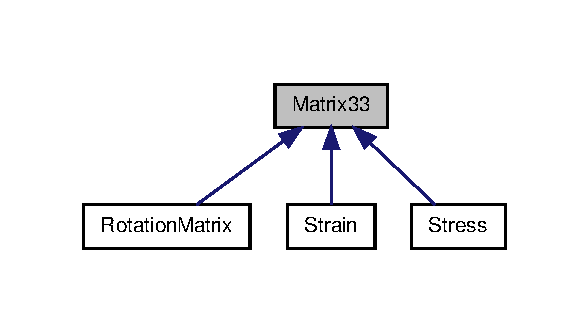
\includegraphics[width=134pt]{dc/dfe/classMatrix33__inherit__graph}
\end{center}
\end{figure}
\subsection*{\-Public \-Member \-Functions}
\begin{DoxyCompactItemize}
\item 
\hyperlink{classMatrix33_a70acb6647b172d017cc4265a29a7d263}{\-Matrix33} ()
\item 
\hyperlink{classMatrix33_a4399c6da8f1ac31ce514550282c823cf}{\-Matrix33} (double $\ast$$\ast$a)
\item 
\hyperlink{classMatrix33_a1f070a29a710043c38b56cee8214e6f7}{\-Matrix33} (\hyperlink{classVector3d}{\-Vector3d} a)
\item 
\hyperlink{classMatrix33_a7f1deae895c26e47c39c76bfaa31d3d2}{\-Matrix33} (\hyperlink{classVector3d}{\-Vector3d} a, \hyperlink{classVector3d}{\-Vector3d} b)
\item 
void \hyperlink{classMatrix33_a6cdcec77fd089b2e73ad7ae85ecff30b}{set\-Value} (int row, int column, double value)
\item 
double \hyperlink{classMatrix33_a849bbdf7b456ddacf7185b087fca4015}{get\-Value} (int row, int column)
\item 
\hyperlink{classMatrix33}{\-Matrix33} \hyperlink{classMatrix33_a4e64ab5af4921c24b8270a0c9050f4ba}{adjugate} ()
\item 
\hyperlink{classMatrix33}{\-Matrix33} \hyperlink{classMatrix33_adc58ec5739c9250ff1150c725d0e868e}{operator+} (const \hyperlink{classMatrix33}{\-Matrix33} \&) const 
\item 
void \hyperlink{classMatrix33_acb59e59d3937e075521f478ba83b7165}{operator+=} (const \hyperlink{classMatrix33}{\-Matrix33} \&)
\item 
\hyperlink{classMatrix33}{\-Matrix33} \hyperlink{classMatrix33_a372f71ec208bb6d3045acd4324b7cb06}{operator-\/} (const \hyperlink{classMatrix33}{\-Matrix33} \&) const 
\item 
void \hyperlink{classMatrix33_abc889e10a9c7c532195c7031c1344a74}{operator-\/=} (const \hyperlink{classMatrix33}{\-Matrix33} \&)
\item 
\hyperlink{classMatrix33}{\-Matrix33} \hyperlink{classMatrix33_a6992fd2bb0b6e9ad71b5d3481c4e3e1a}{operator$\ast$} (const double \&) const 
\item 
void \hyperlink{classMatrix33_a83162791813bef030b1ceb5df3c5cae3}{operator$\ast$=} (const double \&)
\item 
\hyperlink{classMatrix33}{\-Matrix33} \hyperlink{classMatrix33_a525f14614255ff81c0cbab8060e8e065}{operator$\ast$} (const \hyperlink{classMatrix33}{\-Matrix33} \&) const 
\item 
void \hyperlink{classMatrix33_ac3937bdeb034cc83b4adcad16cd58a26}{operator$\ast$=} (const \hyperlink{classMatrix33}{\-Matrix33} \&)
\item 
\hyperlink{classVector3d}{\-Vector3d} \hyperlink{classMatrix33_a601584a1edbaae7c6a2a2874605d6f61}{operator$\ast$} (const \hyperlink{classVector3d}{\-Vector3d} \&) const 
\item 
\hyperlink{classMatrix33}{\-Matrix33} \hyperlink{classMatrix33_ad4ab7b9674a44a297502282e1993ef54}{operator$^\wedge$} () const 
\item 
double \hyperlink{classMatrix33_a15b37caa6ab0d9f4a9f0d95846abd675}{operator$\sim$} () const 
\item 
\hyperlink{classMatrix33}{\-Matrix33} \hyperlink{classMatrix33_a1b822a20343a26b3c9bb7fd5c1247f37}{operator!} () const 
\end{DoxyCompactItemize}
\subsection*{\-Protected \-Attributes}
\begin{DoxyCompactItemize}
\item 
double \hyperlink{classMatrix33_af7f01fa466616eb7c8eda2e4d9f85cdd}{x} \mbox{[}3\mbox{]}\mbox{[}3\mbox{]}
\end{DoxyCompactItemize}


\subsection{\-Detailed \-Description}
\hyperlink{classMatrix33}{\-Matrix33} class representing a 3x3 square matrix. 

\-This class represents a 3x3 square matrix. \-The member functions and operators define various operations that may be carried out on the matrix. 

\-Definition at line 20 of file matrix33.\-h.



\subsection{\-Constructor \& \-Destructor \-Documentation}
\hypertarget{classMatrix33_a70acb6647b172d017cc4265a29a7d263}{\index{\-Matrix33@{\-Matrix33}!\-Matrix33@{\-Matrix33}}
\index{\-Matrix33@{\-Matrix33}!Matrix33@{\-Matrix33}}
\subsubsection[{\-Matrix33}]{\setlength{\rightskip}{0pt plus 5cm}{\bf \-Matrix33\-::\-Matrix33} (
\begin{DoxyParamCaption}
{}
\end{DoxyParamCaption}
)}}\label{de/d82/classMatrix33_a70acb6647b172d017cc4265a29a7d263}
\-Default constructor. 

\-Definition at line 7 of file matrix33.\-cpp.


\begin{DoxyCode}
{
  int i, j;
  
  for (i=0; i<3; i++)
    {
      for (j=0; j<3; j++)
        {
          this->x[i][j] = 0.0;
        }
    }
}
\end{DoxyCode}
\hypertarget{classMatrix33_a4399c6da8f1ac31ce514550282c823cf}{\index{\-Matrix33@{\-Matrix33}!\-Matrix33@{\-Matrix33}}
\index{\-Matrix33@{\-Matrix33}!Matrix33@{\-Matrix33}}
\subsubsection[{\-Matrix33}]{\setlength{\rightskip}{0pt plus 5cm}{\bf \-Matrix33\-::\-Matrix33} (
\begin{DoxyParamCaption}
\item[{double $\ast$$\ast$}]{a}
\end{DoxyParamCaption}
)}}\label{de/d82/classMatrix33_a4399c6da8f1ac31ce514550282c823cf}
\-Constructor with the values provided in a 3x3 matrix. 
\begin{DoxyParams}{\-Parameters}
{\em a} & \-Pointer to the two-\/dimensional 3x3 array. \\
\hline
\end{DoxyParams}


\-Definition at line 24 of file matrix33.\-cpp.


\begin{DoxyCode}
{
  int i, j;
  
  for (i=0; i<3; i++)
    {
      for (j=0; j<3; j++)
        {
          this->x[i][j] = a[i][j];
        }
    }
}
\end{DoxyCode}
\hypertarget{classMatrix33_a1f070a29a710043c38b56cee8214e6f7}{\index{\-Matrix33@{\-Matrix33}!\-Matrix33@{\-Matrix33}}
\index{\-Matrix33@{\-Matrix33}!Matrix33@{\-Matrix33}}
\subsubsection[{\-Matrix33}]{\setlength{\rightskip}{0pt plus 5cm}{\bf \-Matrix33\-::\-Matrix33} (
\begin{DoxyParamCaption}
\item[{{\bf \-Vector3d}}]{a}
\end{DoxyParamCaption}
)}}\label{de/d82/classMatrix33_a1f070a29a710043c38b56cee8214e6f7}
\-Constructor to create the matrix from the dyadic product of a vector with itself. 
\begin{DoxyParams}{\-Parameters}
{\em a} & \-The vector whose dyadic product results in the matrix. \\
\hline
\end{DoxyParams}


\-Definition at line 41 of file matrix33.\-cpp.


\begin{DoxyCode}
{
  int i, j;
  
  for (i=0; i<3; i++)
    {
      for (j=0; j<3; j++)
        {
          this->x[i][j] = a.x[i] * a.x[j];
        }
    }
}
\end{DoxyCode}
\hypertarget{classMatrix33_a7f1deae895c26e47c39c76bfaa31d3d2}{\index{\-Matrix33@{\-Matrix33}!\-Matrix33@{\-Matrix33}}
\index{\-Matrix33@{\-Matrix33}!Matrix33@{\-Matrix33}}
\subsubsection[{\-Matrix33}]{\setlength{\rightskip}{0pt plus 5cm}{\bf \-Matrix33\-::\-Matrix33} (
\begin{DoxyParamCaption}
\item[{{\bf \-Vector3d}}]{a, }
\item[{{\bf \-Vector3d}}]{b}
\end{DoxyParamCaption}
)}}\label{de/d82/classMatrix33_a7f1deae895c26e47c39c76bfaa31d3d2}
\-Constructor with the vectors, the product of which will result in the matrix. 
\begin{DoxyParams}{\-Parameters}
{\em a} & \-First vector. \\
\hline
{\em b} & \-Second vector. \\
\hline
\end{DoxyParams}


\-Definition at line 59 of file matrix33.\-cpp.


\begin{DoxyCode}
{
  int i, j;
  
  for (i=0; i<3; i++)
    {
      for (j=0; j<3; j++)
        {
          this->x[i][j] = a.x[i] * b.x[j];
        }
    }
}
\end{DoxyCode}


\subsection{\-Member \-Function \-Documentation}
\hypertarget{classMatrix33_a4e64ab5af4921c24b8270a0c9050f4ba}{\index{\-Matrix33@{\-Matrix33}!adjugate@{adjugate}}
\index{adjugate@{adjugate}!Matrix33@{\-Matrix33}}
\subsubsection[{adjugate}]{\setlength{\rightskip}{0pt plus 5cm}{\bf \-Matrix33} {\bf \-Matrix33\-::adjugate} (
\begin{DoxyParamCaption}
{}
\end{DoxyParamCaption}
)}}\label{de/d82/classMatrix33_a4e64ab5af4921c24b8270a0c9050f4ba}
\-Returns the adjugate matrix of the present matrix. \begin{DoxyReturn}{\-Returns}
\-The adjugate matrix of the present matrix. 
\end{DoxyReturn}


\-Definition at line 112 of file matrix33.\-cpp.


\begin{DoxyCode}
{
  Matrix33 adj;
  
  adj.x[0][0] = (this->x[1][1]*this->x[2][2]) - (this->x[1][2]*this->x[2][1]);
  adj.x[0][1] = (this->x[1][2]*this->x[2][0]) - (this->x[1][0]*this->x[2][2]);
  adj.x[0][2] = (this->x[1][0]*this->x[2][1]) - (this->x[1][1]*this->x[2][0]);
  
  adj.x[1][0] = (this->x[2][1]*this->x[0][2]) - (this->x[0][1]*this->x[2][2]);
  adj.x[1][1] = (this->x[2][2]*this->x[0][0]) - (this->x[2][0]*this->x[0][2]);
  adj.x[1][2] = (this->x[2][0]*this->x[0][1]) - (this->x[2][1]*this->x[0][0]);
  
  adj.x[2][0] = (this->x[0][1]*this->x[1][2]) - (this->x[0][2]*this->x[1][1]);
  adj.x[2][1] = (this->x[0][2]*this->x[1][0]) - (this->x[0][0]*this->x[1][2]);
  adj.x[2][2] = (this->x[0][0]*this->x[1][1]) - (this->x[1][0]*this->x[0][1]);

  return (adj);
}
\end{DoxyCode}
\hypertarget{classMatrix33_a849bbdf7b456ddacf7185b087fca4015}{\index{\-Matrix33@{\-Matrix33}!get\-Value@{get\-Value}}
\index{get\-Value@{get\-Value}!Matrix33@{\-Matrix33}}
\subsubsection[{get\-Value}]{\setlength{\rightskip}{0pt plus 5cm}double {\bf \-Matrix33\-::get\-Value} (
\begin{DoxyParamCaption}
\item[{int}]{row, }
\item[{int}]{column}
\end{DoxyParamCaption}
)}}\label{de/d82/classMatrix33_a849bbdf7b456ddacf7185b087fca4015}
\-Returns the value of the element located by the row and column indices provided. 
\begin{DoxyParams}{\-Parameters}
{\em row} & \-Row index of the element. \\
\hline
{\em column} & \-Column index of the element. \\
\hline
\end{DoxyParams}
\begin{DoxyReturn}{\-Returns}
\-Value of the element located at the given position.
\end{DoxyReturn}
\-Returns the value of the element located by the row and column indices provided. 
\begin{DoxyParams}{\-Parameters}
{\em row} & \-Row index of the element. \\
\hline
{\em column} & \-Column index of the element. \\
\hline
\end{DoxyParams}


\-Definition at line 95 of file matrix33.\-cpp.


\begin{DoxyCode}
{
  if (row>=0 && row<3)
    {
      if (column>=0 && column<3)
        {
          return (this->x[row][column]);
        }
    }
  
  return (0.0);
}
\end{DoxyCode}
\hypertarget{classMatrix33_a1b822a20343a26b3c9bb7fd5c1247f37}{\index{\-Matrix33@{\-Matrix33}!operator!@{operator!}}
\index{operator!@{operator!}!Matrix33@{\-Matrix33}}
\subsubsection[{operator!}]{\setlength{\rightskip}{0pt plus 5cm}{\bf \-Matrix33} {\bf \-Matrix33\-::operator!} (
\begin{DoxyParamCaption}
{}
\end{DoxyParamCaption}
) const}}\label{de/d82/classMatrix33_a1b822a20343a26b3c9bb7fd5c1247f37}
\-Returns in a new matrix the inverse of the current matrix. \-If the current matrix is non-\/invertible, a zero matrix is returned. 

\-Definition at line 342 of file matrix33.\-cpp.


\begin{DoxyCode}
{
  Matrix33 r;   // Result matrix
  
  double determinant = ~(*this);
  
  if (determinant == 0.0)
    {
      // The matrix is non-invertible
      return (r);       // Zero matrix
    }
  
  // If we are still here, the matrix is invertible
  
  //  Transpose
  Matrix33 tr = ^(*this);
  
  // Find Adjugate matrix
  Matrix33 adj = tr.adjugate();
  
  // Calculate the inverse by dividing the adjugate matrix by the determinant
  r = adj * (1.0/determinant);
  
  return (r);
}
\end{DoxyCode}
\hypertarget{classMatrix33_a6992fd2bb0b6e9ad71b5d3481c4e3e1a}{\index{\-Matrix33@{\-Matrix33}!operator$\ast$@{operator$\ast$}}
\index{operator$\ast$@{operator$\ast$}!Matrix33@{\-Matrix33}}
\subsubsection[{operator$\ast$}]{\setlength{\rightskip}{0pt plus 5cm}{\bf \-Matrix33} \-Matrix33\-::operator$\ast$ (
\begin{DoxyParamCaption}
\item[{const double \&}]{p}
\end{DoxyParamCaption}
) const}}\label{de/d82/classMatrix33_a6992fd2bb0b6e9ad71b5d3481c4e3e1a}
\-Operator for scaling the matrix by a scalar. \-Scales the current matrix by the scalar provided and returns the result in a third matrix. 

\-Definition at line 213 of file matrix33.\-cpp.


\begin{DoxyCode}
{
  int i, j;
  Matrix33 r;
  
  for (i=0; i<3; i++)
    {
      for (j=0; j<3; j++)
        {
          r.x[i][j] = this->x[i][j] * p;
        }
    }
  
  return (r);
}
\end{DoxyCode}
\hypertarget{classMatrix33_a525f14614255ff81c0cbab8060e8e065}{\index{\-Matrix33@{\-Matrix33}!operator$\ast$@{operator$\ast$}}
\index{operator$\ast$@{operator$\ast$}!Matrix33@{\-Matrix33}}
\subsubsection[{operator$\ast$}]{\setlength{\rightskip}{0pt plus 5cm}{\bf \-Matrix33} \-Matrix33\-::operator$\ast$ (
\begin{DoxyParamCaption}
\item[{const {\bf \-Matrix33} \&}]{p}
\end{DoxyParamCaption}
) const}}\label{de/d82/classMatrix33_a525f14614255ff81c0cbab8060e8e065}
\-Operator for the multiplication of two matrices. \-Multiplies the current matrix with another 3x3 matrix and returns the result in a new matrix. 

\-Definition at line 250 of file matrix33.\-cpp.


\begin{DoxyCode}
{
  int i, j, k;
  Matrix33 r;
  
  for (i=0; i<3; i++)
    {
      for (j=0; j<3; j++)
        {
          r.x[i][j] = 0.0;
          for (k=0; k<3; k++)
            {
              r.x[i][j] += this->x[i][k] * p.x[k][j];
            }
        }
    }
  
  return (r);
}
\end{DoxyCode}
\hypertarget{classMatrix33_a601584a1edbaae7c6a2a2874605d6f61}{\index{\-Matrix33@{\-Matrix33}!operator$\ast$@{operator$\ast$}}
\index{operator$\ast$@{operator$\ast$}!Matrix33@{\-Matrix33}}
\subsubsection[{operator$\ast$}]{\setlength{\rightskip}{0pt plus 5cm}{\bf \-Vector3d} \-Matrix33\-::operator$\ast$ (
\begin{DoxyParamCaption}
\item[{const {\bf \-Vector3d} \&}]{v}
\end{DoxyParamCaption}
) const}}\label{de/d82/classMatrix33_a601584a1edbaae7c6a2a2874605d6f61}
\-Returns in a vector the result of the multiplication of the current matrix with the provided vector. 

\-Definition at line 288 of file matrix33.\-cpp.


\begin{DoxyCode}
{
  Vector3d r(0.0, 0.0, 0.0);
  int i, j;
  
  for (i=0; i<3; i++)
    {
      for (j=0; j<3; j++)
        {
          r[i] += this->x[i][j] * v.x[j];
        }
    }
  
  return (r);
}
\end{DoxyCode}
\hypertarget{classMatrix33_a83162791813bef030b1ceb5df3c5cae3}{\index{\-Matrix33@{\-Matrix33}!operator$\ast$=@{operator$\ast$=}}
\index{operator$\ast$=@{operator$\ast$=}!Matrix33@{\-Matrix33}}
\subsubsection[{operator$\ast$=}]{\setlength{\rightskip}{0pt plus 5cm}void \-Matrix33\-::operator$\ast$= (
\begin{DoxyParamCaption}
\item[{const double \&}]{p}
\end{DoxyParamCaption}
)}}\label{de/d82/classMatrix33_a83162791813bef030b1ceb5df3c5cae3}
\-Operator for reflexive scaling of the matrix by a scalar. \-Scales the current matrix by the scalar provided and populates the current matrix elements with the result. 

\-Definition at line 233 of file matrix33.\-cpp.


\begin{DoxyCode}
{
  int i, j;
  
  for (i=0; i<3; i++)
    {
      for (j=0; j<3; j++)
        {
          this->x[i][j] *= p;
        }
    }
}
\end{DoxyCode}
\hypertarget{classMatrix33_ac3937bdeb034cc83b4adcad16cd58a26}{\index{\-Matrix33@{\-Matrix33}!operator$\ast$=@{operator$\ast$=}}
\index{operator$\ast$=@{operator$\ast$=}!Matrix33@{\-Matrix33}}
\subsubsection[{operator$\ast$=}]{\setlength{\rightskip}{0pt plus 5cm}void \-Matrix33\-::operator$\ast$= (
\begin{DoxyParamCaption}
\item[{const {\bf \-Matrix33} \&}]{p}
\end{DoxyParamCaption}
)}}\label{de/d82/classMatrix33_ac3937bdeb034cc83b4adcad16cd58a26}
\-Operator for reflexive multiplication of two matrices. \-Multiplies the current matrix with another 3x3 matrix and populates the elements of the current matrix with the result. 

\-Definition at line 274 of file matrix33.\-cpp.


\begin{DoxyCode}
{
  Matrix33* r = new Matrix33;
  
  *r = (*this) * p;
  *this = *r;
  
  delete(r);
  r = NULL;
}
\end{DoxyCode}
\hypertarget{classMatrix33_adc58ec5739c9250ff1150c725d0e868e}{\index{\-Matrix33@{\-Matrix33}!operator+@{operator+}}
\index{operator+@{operator+}!Matrix33@{\-Matrix33}}
\subsubsection[{operator+}]{\setlength{\rightskip}{0pt plus 5cm}{\bf \-Matrix33} \-Matrix33\-::operator+ (
\begin{DoxyParamCaption}
\item[{const {\bf \-Matrix33} \&}]{p}
\end{DoxyParamCaption}
) const}}\label{de/d82/classMatrix33_adc58ec5739c9250ff1150c725d0e868e}
\-Operator for addition of two matrices. \-Adds the current matrix to the provided matrix and returns a third matrix with the result. 

\-Definition at line 137 of file matrix33.\-cpp.


\begin{DoxyCode}
{
  int i, j;
  Matrix33 r;
  
  for (i=0; i<3; i++)
    {
      for (j=0; j<3; j++)
        {
          r.x[i][j] = this->x[i][j] + p.x[i][j];
        }
    }
  
  return (r);
}
\end{DoxyCode}
\hypertarget{classMatrix33_acb59e59d3937e075521f478ba83b7165}{\index{\-Matrix33@{\-Matrix33}!operator+=@{operator+=}}
\index{operator+=@{operator+=}!Matrix33@{\-Matrix33}}
\subsubsection[{operator+=}]{\setlength{\rightskip}{0pt plus 5cm}void \-Matrix33\-::operator+= (
\begin{DoxyParamCaption}
\item[{const {\bf \-Matrix33} \&}]{p}
\end{DoxyParamCaption}
)}}\label{de/d82/classMatrix33_acb59e59d3937e075521f478ba83b7165}
\-Operator for reflexive addition of two matrices. \-Adds the current matrix to the provided matrix and populates the current matrix elements with the result. 

\-Definition at line 157 of file matrix33.\-cpp.


\begin{DoxyCode}
{
  int i, j;
  
  for (i=0; i<3; i++)
    {
      for (j=0; j<3; j++)
        {
          this->x[i][j] += p.x[i][j];
        }
    }
}
\end{DoxyCode}
\hypertarget{classMatrix33_a372f71ec208bb6d3045acd4324b7cb06}{\index{\-Matrix33@{\-Matrix33}!operator-\/@{operator-\/}}
\index{operator-\/@{operator-\/}!Matrix33@{\-Matrix33}}
\subsubsection[{operator-\/}]{\setlength{\rightskip}{0pt plus 5cm}{\bf \-Matrix33} \-Matrix33\-::operator-\/ (
\begin{DoxyParamCaption}
\item[{const {\bf \-Matrix33} \&}]{p}
\end{DoxyParamCaption}
) const}}\label{de/d82/classMatrix33_a372f71ec208bb6d3045acd4324b7cb06}
\-Operator for the subtraction of two matrices. \-Subtracts the given matrix from the current matrix and returns the result in a new matrix. 

\-Definition at line 175 of file matrix33.\-cpp.


\begin{DoxyCode}
{
  int i, j;
  Matrix33 r;
  
  for (i=0; i<3; i++)
    {
      for (j=0; j<3; j++)
        {
          r.x[i][j] = this->x[i][j] - p.x[i][j];
        }
    }
  
  return (r);
}
\end{DoxyCode}
\hypertarget{classMatrix33_abc889e10a9c7c532195c7031c1344a74}{\index{\-Matrix33@{\-Matrix33}!operator-\/=@{operator-\/=}}
\index{operator-\/=@{operator-\/=}!Matrix33@{\-Matrix33}}
\subsubsection[{operator-\/=}]{\setlength{\rightskip}{0pt plus 5cm}void \-Matrix33\-::operator-\/= (
\begin{DoxyParamCaption}
\item[{const {\bf \-Matrix33} \&}]{p}
\end{DoxyParamCaption}
)}}\label{de/d82/classMatrix33_abc889e10a9c7c532195c7031c1344a74}
\-Operator for reflexive subtraction of two matrices. \-Subtracts the given matrix from the current matrix and populates the current matrix with the result. 

\-Definition at line 195 of file matrix33.\-cpp.


\begin{DoxyCode}
{
  int i, j;
  
  for (i=0; i<3; i++)
    {
      for (j=0; j<3; j++)
        {
          this->x[i][j] -= p.x[i][j];
        }
    }
}
\end{DoxyCode}
\hypertarget{classMatrix33_ad4ab7b9674a44a297502282e1993ef54}{\index{\-Matrix33@{\-Matrix33}!operator$^\wedge$@{operator$^\wedge$}}
\index{operator$^\wedge$@{operator$^\wedge$}!Matrix33@{\-Matrix33}}
\subsubsection[{operator$^\wedge$}]{\setlength{\rightskip}{0pt plus 5cm}{\bf \-Matrix33} \-Matrix33\-::operator$^\wedge$ (
\begin{DoxyParamCaption}
{}
\end{DoxyParamCaption}
) const}}\label{de/d82/classMatrix33_ad4ab7b9674a44a297502282e1993ef54}
\-Returns in a new matrix the transpose of the current matrix. 

\-Definition at line 308 of file matrix33.\-cpp.


\begin{DoxyCode}
{
  Matrix33 r;
  int i, j;
  
  for (i=0; i<3; i++)
    {
      for (j=0; j<3; j++)
        {
          r.x[i][j] = this->x[j][i];
        }
    }
  
  return (r);
}
\end{DoxyCode}
\hypertarget{classMatrix33_a15b37caa6ab0d9f4a9f0d95846abd675}{\index{\-Matrix33@{\-Matrix33}!operator$\sim$@{operator$\sim$}}
\index{operator$\sim$@{operator$\sim$}!Matrix33@{\-Matrix33}}
\subsubsection[{operator$\sim$}]{\setlength{\rightskip}{0pt plus 5cm}double {\bf \-Matrix33\-::operator$\sim$} (
\begin{DoxyParamCaption}
{}
\end{DoxyParamCaption}
) const}}\label{de/d82/classMatrix33_a15b37caa6ab0d9f4a9f0d95846abd675}
\-Returns the determinant of the current matrix. 

\-Definition at line 327 of file matrix33.\-cpp.


\begin{DoxyCode}
{
  double d = 0.0;
  
  d += this.x[0][0] * ( (this->x[1][1]*this->x[2][2]) - (this->x[2][1]*this->x[
      1][2]) );
  d += this.x[0][1] * ( (this->x[1][2]*this->x[2][0]) - (this->x[1][0]*this->x[
      2][2]) );
  d += this.x[0][2] * ( (this->x[1][0]*this->x[2][1]) - (this->x[2][0]*this->x[
      1][1]) );
  
  return (d);
}
\end{DoxyCode}
\hypertarget{classMatrix33_a6cdcec77fd089b2e73ad7ae85ecff30b}{\index{\-Matrix33@{\-Matrix33}!set\-Value@{set\-Value}}
\index{set\-Value@{set\-Value}!Matrix33@{\-Matrix33}}
\subsubsection[{set\-Value}]{\setlength{\rightskip}{0pt plus 5cm}void {\bf \-Matrix33\-::set\-Value} (
\begin{DoxyParamCaption}
\item[{int}]{row, }
\item[{int}]{column, }
\item[{double}]{value}
\end{DoxyParamCaption}
)}}\label{de/d82/classMatrix33_a6cdcec77fd089b2e73ad7ae85ecff30b}
\-Function to set the value of an element indicated by its position. 
\begin{DoxyParams}{\-Parameters}
{\em row} & \-Row index of the element. \\
\hline
{\em column} & \-Column index of the element. \\
\hline
{\em value} & \-Value that the element is to be set to. \\
\hline
\end{DoxyParams}


\-Definition at line 79 of file matrix33.\-cpp.


\begin{DoxyCode}
{
  if (row>=0 && row<3)
    {
      if (column>=0 && column<3)
        {
          this->x[row][column] = value;
        }
    }
}
\end{DoxyCode}


\subsection{\-Field \-Documentation}
\hypertarget{classMatrix33_af7f01fa466616eb7c8eda2e4d9f85cdd}{\index{\-Matrix33@{\-Matrix33}!x@{x}}
\index{x@{x}!Matrix33@{\-Matrix33}}
\subsubsection[{x}]{\setlength{\rightskip}{0pt plus 5cm}double {\bf \-Matrix33\-::x}\mbox{[}3\mbox{]}\mbox{[}3\mbox{]}\hspace{0.3cm}{\ttfamily  \mbox{[}protected\mbox{]}}}}\label{de/d82/classMatrix33_af7f01fa466616eb7c8eda2e4d9f85cdd}
\-Array containing the elements of the matrix. 

\-Definition at line 26 of file matrix33.\-h.



\-The documentation for this class was generated from the following files\-:\begin{DoxyCompactItemize}
\item 
\hyperlink{matrix33_8h}{matrix33.\-h}\item 
\hyperlink{matrix33_8cpp}{matrix33.\-cpp}\end{DoxyCompactItemize}

\hypertarget{classStress}{\section{\-Stress \-Class \-Reference}
\label{d1/d1c/classStress}\index{\-Stress@{\-Stress}}
}


\hyperlink{classStress}{\-Stress} class to represent the stress tensor.  




{\ttfamily \#include $<$stress.\-h$>$}



\-Inheritance diagram for \-Stress\-:
\nopagebreak
\begin{figure}[H]
\begin{center}
\leavevmode
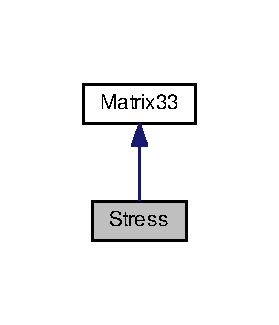
\includegraphics[width=134pt]{dd/d46/classStress__inherit__graph}
\end{center}
\end{figure}


\-Collaboration diagram for \-Stress\-:
\nopagebreak
\begin{figure}[H]
\begin{center}
\leavevmode
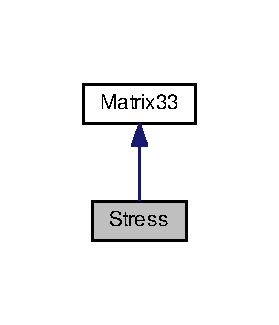
\includegraphics[width=134pt]{d7/dfa/classStress__coll__graph}
\end{center}
\end{figure}
\subsection*{\-Public \-Member \-Functions}
\begin{DoxyCompactItemize}
\item 
\hyperlink{classStress_aa01e83a3f6791cbadc5a368e3a40515e}{\-Stress} ()
\begin{DoxyCompactList}\small\item\em \-Default constructor. \end{DoxyCompactList}\item 
\hyperlink{classStress_ae4e2f6250e3bdd4d3d78a9c6bdde7bab}{\-Stress} (double $\ast$principal, double $\ast$shear)
\begin{DoxyCompactList}\small\item\em \-Constructor specifying the principal and shear stresses. \end{DoxyCompactList}\item 
void \hyperlink{classStress_aa395d5763df8feb4689e0c5524c9e562}{populate\-Matrix} ()
\begin{DoxyCompactList}\small\item\em \-Construct the stress tensor from the principal and shear stresses. \end{DoxyCompactList}\item 
double $\ast$ \hyperlink{classStress_aca57d2719f43701dd2ebf2ab00afa539}{get\-Principal\-Stresses} ()
\begin{DoxyCompactList}\small\item\em \-Get the principal stresses. \end{DoxyCompactList}\item 
double $\ast$ \hyperlink{classStress_afe8214b8e9061930e6598e1970fd61f5}{get\-Shear\-Stresses} ()
\begin{DoxyCompactList}\small\item\em \-Get the shear stresses. \end{DoxyCompactList}\item 
\hyperlink{classStress}{\-Stress} \hyperlink{classStress_a61fa75450c0232bb0fa427072d1b6a35}{rotate} (\hyperlink{classMatrix33}{\-Matrix33} alpha)
\begin{DoxyCompactList}\small\item\em \-Rotate the stress tensor from one coordinate system to another. \end{DoxyCompactList}\item 
void \hyperlink{classMatrix33_a6cdcec77fd089b2e73ad7ae85ecff30b}{set\-Value} (int row, int column, double value)
\begin{DoxyCompactList}\small\item\em \-Function to set the value of an element indicated by its position. \end{DoxyCompactList}\item 
double \hyperlink{classMatrix33_a849bbdf7b456ddacf7185b087fca4015}{get\-Value} (int row, int column)
\begin{DoxyCompactList}\small\item\em \-Returns the value of the element located by the row and column indices provided. \end{DoxyCompactList}\item 
\hyperlink{classMatrix33}{\-Matrix33} \hyperlink{classMatrix33_a4e64ab5af4921c24b8270a0c9050f4ba}{adjugate} ()
\begin{DoxyCompactList}\small\item\em \-Returns the adjugate matrix of the present matrix. \end{DoxyCompactList}\item 
\hyperlink{classMatrix33}{\-Matrix33} \hyperlink{classMatrix33_adc58ec5739c9250ff1150c725d0e868e}{operator+} (const \hyperlink{classMatrix33}{\-Matrix33} \&) const 
\begin{DoxyCompactList}\small\item\em \-Operator for addition of two matrices. \end{DoxyCompactList}\item 
void \hyperlink{classMatrix33_acb59e59d3937e075521f478ba83b7165}{operator+=} (const \hyperlink{classMatrix33}{\-Matrix33} \&)
\begin{DoxyCompactList}\small\item\em \-Operator for reflexive addition of two matrices. \end{DoxyCompactList}\item 
\hyperlink{classMatrix33}{\-Matrix33} \hyperlink{classMatrix33_a372f71ec208bb6d3045acd4324b7cb06}{operator-\/} (const \hyperlink{classMatrix33}{\-Matrix33} \&) const 
\begin{DoxyCompactList}\small\item\em \-Operator for the subtraction of two matrices. \end{DoxyCompactList}\item 
void \hyperlink{classMatrix33_abc889e10a9c7c532195c7031c1344a74}{operator-\/=} (const \hyperlink{classMatrix33}{\-Matrix33} \&)
\begin{DoxyCompactList}\small\item\em \-Operator for reflexive subtraction of two matrices. \end{DoxyCompactList}\item 
\hyperlink{classMatrix33}{\-Matrix33} \hyperlink{classMatrix33_a6992fd2bb0b6e9ad71b5d3481c4e3e1a}{operator$\ast$} (const double \&) const 
\begin{DoxyCompactList}\small\item\em \-Operator for scaling the matrix by a scalar. \end{DoxyCompactList}\item 
\hyperlink{classMatrix33}{\-Matrix33} \hyperlink{classMatrix33_a525f14614255ff81c0cbab8060e8e065}{operator$\ast$} (const \hyperlink{classMatrix33}{\-Matrix33} \&) const 
\begin{DoxyCompactList}\small\item\em \-Operator for the multiplication of two matrices. \end{DoxyCompactList}\item 
\hyperlink{classVector3d}{\-Vector3d} \hyperlink{classMatrix33_a601584a1edbaae7c6a2a2874605d6f61}{operator$\ast$} (const \hyperlink{classVector3d}{\-Vector3d} \&) const 
\begin{DoxyCompactList}\small\item\em \-Operator for the multiplication of a matrix with a vector. \end{DoxyCompactList}\item 
void \hyperlink{classMatrix33_a83162791813bef030b1ceb5df3c5cae3}{operator$\ast$=} (const double \&)
\begin{DoxyCompactList}\small\item\em \-Operator for reflexive scaling of the matrix by a scalar. \end{DoxyCompactList}\item 
void \hyperlink{classMatrix33_ac3937bdeb034cc83b4adcad16cd58a26}{operator$\ast$=} (const \hyperlink{classMatrix33}{\-Matrix33} \&)
\begin{DoxyCompactList}\small\item\em \-Operator for reflexive multiplication of two matrices. \end{DoxyCompactList}\item 
\hyperlink{classMatrix33}{\-Matrix33} \hyperlink{classMatrix33_ad4ab7b9674a44a297502282e1993ef54}{operator$^\wedge$} () const 
\begin{DoxyCompactList}\small\item\em \-Transpose. \end{DoxyCompactList}\item 
double \hyperlink{classMatrix33_a15b37caa6ab0d9f4a9f0d95846abd675}{operator$\sim$} () const 
\begin{DoxyCompactList}\small\item\em \-Determinant. \end{DoxyCompactList}\item 
\hyperlink{classMatrix33}{\-Matrix33} \hyperlink{classMatrix33_a1b822a20343a26b3c9bb7fd5c1247f37}{operator!} () const 
\begin{DoxyCompactList}\small\item\em \-Inverse. \end{DoxyCompactList}\end{DoxyCompactItemize}
\subsection*{\-Protected \-Attributes}
\begin{DoxyCompactItemize}
\item 
double \hyperlink{classStress_aea8c3e40aa59a89d7ba79d2c916050a6}{principal\-Stresses} \mbox{[}3\mbox{]}
\item 
double \hyperlink{classStress_a77e8705e56c2fb56826a638edf3f78bf}{shear\-Stresses} \mbox{[}3\mbox{]}
\item 
double \hyperlink{classMatrix33_af7f01fa466616eb7c8eda2e4d9f85cdd}{x} \mbox{[}3\mbox{]}\mbox{[}3\mbox{]}
\begin{DoxyCompactList}\small\item\em \-Array containing the elements of the matrix. \end{DoxyCompactList}\end{DoxyCompactItemize}


\subsection{\-Detailed \-Description}
\hyperlink{classStress}{\-Stress} class to represent the stress tensor. 

\-The member functions of this class construct the symmetric stress tensor and operate on it. 

\-Definition at line 20 of file stress.\-h.



\subsection{\-Constructor \& \-Destructor \-Documentation}
\hypertarget{classStress_aa01e83a3f6791cbadc5a368e3a40515e}{\index{\-Stress@{\-Stress}!\-Stress@{\-Stress}}
\index{\-Stress@{\-Stress}!Stress@{\-Stress}}
\subsubsection[{\-Stress}]{\setlength{\rightskip}{0pt plus 5cm}{\bf \-Stress\-::\-Stress} (
\begin{DoxyParamCaption}
{}
\end{DoxyParamCaption}
)}}\label{d1/d1c/classStress_aa01e83a3f6791cbadc5a368e3a40515e}


\-Default constructor. 

\-Initializes the stress tensor with zeros. 

\-Definition at line 16 of file stress.\-cpp.


\begin{DoxyCode}
{
  int i, j;
  
  for (i=0; i<3; i++)
    {
      principalStresses [i] = 0.0;
      shearStresses [i] = 0.0;
    }

  this->populateMatrix ();
}
\end{DoxyCode}
\hypertarget{classStress_ae4e2f6250e3bdd4d3d78a9c6bdde7bab}{\index{\-Stress@{\-Stress}!\-Stress@{\-Stress}}
\index{\-Stress@{\-Stress}!Stress@{\-Stress}}
\subsubsection[{\-Stress}]{\setlength{\rightskip}{0pt plus 5cm}{\bf \-Stress\-::\-Stress} (
\begin{DoxyParamCaption}
\item[{double $\ast$}]{principal, }
\item[{double $\ast$}]{shear}
\end{DoxyParamCaption}
)}}\label{d1/d1c/classStress_ae4e2f6250e3bdd4d3d78a9c6bdde7bab}


\-Constructor specifying the principal and shear stresses. 

\-The principal and shear stresses are provided in the arguments and the symmetrical stress tensor is contstructed using them. 
\begin{DoxyParams}{\-Parameters}
{\em principal} & \-Pointer to the array containing principal stresses. \\
\hline
{\em shear} & \-Pointer to the array containing shear stresses. \\
\hline
\end{DoxyParams}


\-Definition at line 35 of file stress.\-cpp.


\begin{DoxyCode}
{
  int i;
  
  for (i=0; i<3; i++)
    {
      this->principalStresses [i] = principal [i];
      this->shearStresses [i] = shear [i];
    }
  
  this->populateMatrix ();
}
\end{DoxyCode}


\subsection{\-Member \-Function \-Documentation}
\hypertarget{classMatrix33_a4e64ab5af4921c24b8270a0c9050f4ba}{\index{\-Stress@{\-Stress}!adjugate@{adjugate}}
\index{adjugate@{adjugate}!Stress@{\-Stress}}
\subsubsection[{adjugate}]{\setlength{\rightskip}{0pt plus 5cm}{\bf \-Matrix33} {\bf \-Matrix33\-::adjugate} (
\begin{DoxyParamCaption}
{}
\end{DoxyParamCaption}
)\hspace{0.3cm}{\ttfamily  \mbox{[}inherited\mbox{]}}}}\label{de/d82/classMatrix33_a4e64ab5af4921c24b8270a0c9050f4ba}


\-Returns the adjugate matrix of the present matrix. 

\-The adjugate matrix of the present matrix is returned. \-The adjugate matrix is calculated by evaluating the determinant of the cofactor matrix of each element, and then replacing the corresponding element position by the value of the determinant. \-This operation is useful in calculating the inverse of a matrix. \begin{DoxyReturn}{\-Returns}
\-The adjugate matrix of the present matrix. 
\end{DoxyReturn}


\-Definition at line 129 of file matrix33.\-cpp.


\begin{DoxyCode}
{
  Matrix33 adj;
  
  adj.x[0][0] = (this->x[1][1]*this->x[2][2]) - (this->x[1][2]*this->x[2][1]);
  adj.x[0][1] = (this->x[1][2]*this->x[2][0]) - (this->x[1][0]*this->x[2][2]);
  adj.x[0][2] = (this->x[1][0]*this->x[2][1]) - (this->x[1][1]*this->x[2][0]);
  
  adj.x[1][0] = (this->x[2][1]*this->x[0][2]) - (this->x[0][1]*this->x[2][2]);
  adj.x[1][1] = (this->x[2][2]*this->x[0][0]) - (this->x[2][0]*this->x[0][2]);
  adj.x[1][2] = (this->x[2][0]*this->x[0][1]) - (this->x[2][1]*this->x[0][0]);
  
  adj.x[2][0] = (this->x[0][1]*this->x[1][2]) - (this->x[0][2]*this->x[1][1]);
  adj.x[2][1] = (this->x[0][2]*this->x[1][0]) - (this->x[0][0]*this->x[1][2]);
  adj.x[2][2] = (this->x[0][0]*this->x[1][1]) - (this->x[1][0]*this->x[0][1]);

  return (adj);
}
\end{DoxyCode}
\hypertarget{classStress_aca57d2719f43701dd2ebf2ab00afa539}{\index{\-Stress@{\-Stress}!get\-Principal\-Stresses@{get\-Principal\-Stresses}}
\index{get\-Principal\-Stresses@{get\-Principal\-Stresses}!Stress@{\-Stress}}
\subsubsection[{get\-Principal\-Stresses}]{\setlength{\rightskip}{0pt plus 5cm}double $\ast$ {\bf \-Stress\-::get\-Principal\-Stresses} (
\begin{DoxyParamCaption}
{}
\end{DoxyParamCaption}
)}}\label{d1/d1c/classStress_aca57d2719f43701dd2ebf2ab00afa539}


\-Get the principal stresses. 

\-Returns a 3-\/member array with the principal stresses\-: s11 s22 s33. \begin{DoxyReturn}{\-Returns}
3-\/member array with the principal stresses. 
\end{DoxyReturn}


\-Definition at line 68 of file stress.\-cpp.


\begin{DoxyCode}
{
  double p[3];
  int i;
  
  for (i=0; i<3; i++)
    {
      p[i] = this->principalStresses[i];
    }
  
  return (p);
}
\end{DoxyCode}
\hypertarget{classStress_afe8214b8e9061930e6598e1970fd61f5}{\index{\-Stress@{\-Stress}!get\-Shear\-Stresses@{get\-Shear\-Stresses}}
\index{get\-Shear\-Stresses@{get\-Shear\-Stresses}!Stress@{\-Stress}}
\subsubsection[{get\-Shear\-Stresses}]{\setlength{\rightskip}{0pt plus 5cm}double $\ast$ {\bf \-Stress\-::get\-Shear\-Stresses} (
\begin{DoxyParamCaption}
{}
\end{DoxyParamCaption}
)}}\label{d1/d1c/classStress_afe8214b8e9061930e6598e1970fd61f5}


\-Get the shear stresses. 

\-Returns a 3-\/member array with the shear stresses\-: s12 s13 s23. \begin{DoxyReturn}{\-Returns}
3-\/member array with the shear stresses. 
\end{DoxyReturn}


\-Definition at line 86 of file stress.\-cpp.


\begin{DoxyCode}
{
  double s[3];
  int i;
  
  for (i=0; i<3; i++)
    {
      s[i] = this->shearStresses[i];
    }
  
  return (s);
}
\end{DoxyCode}
\hypertarget{classMatrix33_a849bbdf7b456ddacf7185b087fca4015}{\index{\-Stress@{\-Stress}!get\-Value@{get\-Value}}
\index{get\-Value@{get\-Value}!Stress@{\-Stress}}
\subsubsection[{get\-Value}]{\setlength{\rightskip}{0pt plus 5cm}double {\bf \-Matrix33\-::get\-Value} (
\begin{DoxyParamCaption}
\item[{int}]{row, }
\item[{int}]{column}
\end{DoxyParamCaption}
)\hspace{0.3cm}{\ttfamily  \mbox{[}inherited\mbox{]}}}}\label{de/d82/classMatrix33_a849bbdf7b456ddacf7185b087fca4015}


\-Returns the value of the element located by the row and column indices provided. 

\-The value of the element indicated by the arguments row and column is returned. \-The values of row and column must correspond to array indices, and thus can be one of 0, 1 and 2. \-In any other case 0.\-0 is returned. 
\begin{DoxyParams}{\-Parameters}
{\em row} & \-Row index of the element. \\
\hline
{\em column} & \-Column index of the element. \\
\hline
\end{DoxyParams}
\begin{DoxyReturn}{\-Returns}
\-Value of the element located at the given position. 
\end{DoxyReturn}


\-Definition at line 111 of file matrix33.\-cpp.


\begin{DoxyCode}
{
  if (row>=0 && row<3)
    {
      if (column>=0 && column<3)
        {
          return (this->x[row][column]);
        }
    }
  
  return (0.0);
}
\end{DoxyCode}
\hypertarget{classMatrix33_a1b822a20343a26b3c9bb7fd5c1247f37}{\index{\-Stress@{\-Stress}!operator!@{operator!}}
\index{operator!@{operator!}!Stress@{\-Stress}}
\subsubsection[{operator!}]{\setlength{\rightskip}{0pt plus 5cm}{\bf \-Matrix33} {\bf \-Matrix33\-::operator!} (
\begin{DoxyParamCaption}
{}
\end{DoxyParamCaption}
) const\hspace{0.3cm}{\ttfamily  \mbox{[}inherited\mbox{]}}}}\label{de/d82/classMatrix33_a1b822a20343a26b3c9bb7fd5c1247f37}


\-Inverse. 

\-Returns in a new matrix the inverse of the current matrix. \-If the current matrix is non-\/invertible, a zero matrix is returned. \begin{DoxyReturn}{\-Returns}
\-Matrix with the inverse of the current matrix. \-If the current matrix is non-\/invertible, a zero matrix is returned. 
\end{DoxyReturn}


\-Definition at line 370 of file matrix33.\-cpp.


\begin{DoxyCode}
{
  Matrix33 r;   // Result matrix
  
  double determinant = ~(*this);
  
  if (determinant == 0.0)
    {
      // The matrix is non-invertible
      return (r);       // Zero matrix
    }
  
  // If we are still here, the matrix is invertible
  
  //  Transpose
  Matrix33 tr = ^(*this);
  
  // Find Adjugate matrix
  Matrix33 adj = tr.adjugate();
  
  // Calculate the inverse by dividing the adjugate matrix by the determinant
  r = adj * (1.0/determinant);
  
  return (r);
}
\end{DoxyCode}
\hypertarget{classMatrix33_a6992fd2bb0b6e9ad71b5d3481c4e3e1a}{\index{\-Stress@{\-Stress}!operator$\ast$@{operator$\ast$}}
\index{operator$\ast$@{operator$\ast$}!Stress@{\-Stress}}
\subsubsection[{operator$\ast$}]{\setlength{\rightskip}{0pt plus 5cm}{\bf \-Matrix33} \-Matrix33\-::operator$\ast$ (
\begin{DoxyParamCaption}
\item[{const double \&}]{p}
\end{DoxyParamCaption}
) const\hspace{0.3cm}{\ttfamily  \mbox{[}inherited\mbox{]}}}}\label{de/d82/classMatrix33_a6992fd2bb0b6e9ad71b5d3481c4e3e1a}


\-Operator for scaling the matrix by a scalar. 

\-Scales the current matrix by the scalar provided and returns the result in a third matrix. \begin{DoxyReturn}{\-Returns}
\-Matrix containing the result of scaling the current matrix by the scalar provided as argument. 
\end{DoxyReturn}


\-Definition at line 233 of file matrix33.\-cpp.


\begin{DoxyCode}
{
  int i, j;
  Matrix33 r;
  
  for (i=0; i<3; i++)
    {
      for (j=0; j<3; j++)
        {
          r.x[i][j] = this->x[i][j] * p;
        }
    }
  
  return (r);
}
\end{DoxyCode}
\hypertarget{classMatrix33_a525f14614255ff81c0cbab8060e8e065}{\index{\-Stress@{\-Stress}!operator$\ast$@{operator$\ast$}}
\index{operator$\ast$@{operator$\ast$}!Stress@{\-Stress}}
\subsubsection[{operator$\ast$}]{\setlength{\rightskip}{0pt plus 5cm}{\bf \-Matrix33} \-Matrix33\-::operator$\ast$ (
\begin{DoxyParamCaption}
\item[{const {\bf \-Matrix33} \&}]{p}
\end{DoxyParamCaption}
) const\hspace{0.3cm}{\ttfamily  \mbox{[}inherited\mbox{]}}}}\label{de/d82/classMatrix33_a525f14614255ff81c0cbab8060e8e065}


\-Operator for the multiplication of two matrices. 

\-Multiplies the current matrix with another 3x3 matrix and returns the result in a new matrix. \begin{DoxyReturn}{\-Returns}
\-The result of the multiplication of the current matrix with the one provided as argument. 
\end{DoxyReturn}


\-Definition at line 271 of file matrix33.\-cpp.


\begin{DoxyCode}
{
  int i, j, k;
  Matrix33 r;
  
  for (i=0; i<3; i++)
    {
      for (j=0; j<3; j++)
        {
          r.x[i][j] = 0.0;
          for (k=0; k<3; k++)
            {
              r.x[i][j] += this->x[i][k] * p.x[k][j];
            }
        }
    }
  
  return (r);
}
\end{DoxyCode}
\hypertarget{classMatrix33_a601584a1edbaae7c6a2a2874605d6f61}{\index{\-Stress@{\-Stress}!operator$\ast$@{operator$\ast$}}
\index{operator$\ast$@{operator$\ast$}!Stress@{\-Stress}}
\subsubsection[{operator$\ast$}]{\setlength{\rightskip}{0pt plus 5cm}{\bf \-Vector3d} \-Matrix33\-::operator$\ast$ (
\begin{DoxyParamCaption}
\item[{const {\bf \-Vector3d} \&}]{v}
\end{DoxyParamCaption}
) const\hspace{0.3cm}{\ttfamily  \mbox{[}inherited\mbox{]}}}}\label{de/d82/classMatrix33_a601584a1edbaae7c6a2a2874605d6f61}


\-Operator for the multiplication of a matrix with a vector. 

\-Returns in a vector the result of the multiplication of the current matrix with the provided vector. \begin{DoxyReturn}{\-Returns}
\-The vector resulting from the multiplication of the current matrix with a vector. 
\end{DoxyReturn}


\-Definition at line 311 of file matrix33.\-cpp.


\begin{DoxyCode}
{
  Vector3d r(0.0, 0.0, 0.0);
  int i, j;
  
  for (i=0; i<3; i++)
    {
      for (j=0; j<3; j++)
        {
          r[i] += this->x[i][j] * v.x[j];
        }
    }
  
  return (r);
}
\end{DoxyCode}
\hypertarget{classMatrix33_a83162791813bef030b1ceb5df3c5cae3}{\index{\-Stress@{\-Stress}!operator$\ast$=@{operator$\ast$=}}
\index{operator$\ast$=@{operator$\ast$=}!Stress@{\-Stress}}
\subsubsection[{operator$\ast$=}]{\setlength{\rightskip}{0pt plus 5cm}void \-Matrix33\-::operator$\ast$= (
\begin{DoxyParamCaption}
\item[{const double \&}]{p}
\end{DoxyParamCaption}
)\hspace{0.3cm}{\ttfamily  \mbox{[}inherited\mbox{]}}}}\label{de/d82/classMatrix33_a83162791813bef030b1ceb5df3c5cae3}


\-Operator for reflexive scaling of the matrix by a scalar. 

\-Scales the current matrix by the scalar provided and populates the current matrix elements with the result. 

\-Definition at line 253 of file matrix33.\-cpp.


\begin{DoxyCode}
{
  int i, j;
  
  for (i=0; i<3; i++)
    {
      for (j=0; j<3; j++)
        {
          this->x[i][j] *= p;
        }
    }
}
\end{DoxyCode}
\hypertarget{classMatrix33_ac3937bdeb034cc83b4adcad16cd58a26}{\index{\-Stress@{\-Stress}!operator$\ast$=@{operator$\ast$=}}
\index{operator$\ast$=@{operator$\ast$=}!Stress@{\-Stress}}
\subsubsection[{operator$\ast$=}]{\setlength{\rightskip}{0pt plus 5cm}void \-Matrix33\-::operator$\ast$= (
\begin{DoxyParamCaption}
\item[{const {\bf \-Matrix33} \&}]{p}
\end{DoxyParamCaption}
)\hspace{0.3cm}{\ttfamily  \mbox{[}inherited\mbox{]}}}}\label{de/d82/classMatrix33_ac3937bdeb034cc83b4adcad16cd58a26}


\-Operator for reflexive multiplication of two matrices. 

\-Multiplies the current matrix with another 3x3 matrix and populates the elements of the current matrix with the result. 

\-Definition at line 295 of file matrix33.\-cpp.


\begin{DoxyCode}
{
  Matrix33* r = new Matrix33;
  
  *r = (*this) * p;
  *this = *r;
  
  delete(r);
  r = NULL;
}
\end{DoxyCode}
\hypertarget{classMatrix33_adc58ec5739c9250ff1150c725d0e868e}{\index{\-Stress@{\-Stress}!operator+@{operator+}}
\index{operator+@{operator+}!Stress@{\-Stress}}
\subsubsection[{operator+}]{\setlength{\rightskip}{0pt plus 5cm}{\bf \-Matrix33} \-Matrix33\-::operator+ (
\begin{DoxyParamCaption}
\item[{const {\bf \-Matrix33} \&}]{p}
\end{DoxyParamCaption}
) const\hspace{0.3cm}{\ttfamily  \mbox{[}inherited\mbox{]}}}}\label{de/d82/classMatrix33_adc58ec5739c9250ff1150c725d0e868e}


\-Operator for addition of two matrices. 

\-Adds the current matrix to the provided matrix and returns a third matrix with the result. \begin{DoxyReturn}{\-Returns}
\-Matrix containing the sum of the present matrix and the one provided. 
\end{DoxyReturn}


\-Definition at line 155 of file matrix33.\-cpp.


\begin{DoxyCode}
{
  int i, j;
  Matrix33 r;
  
  for (i=0; i<3; i++)
    {
      for (j=0; j<3; j++)
        {
          r.x[i][j] = this->x[i][j] + p.x[i][j];
        }
    }
  
  return (r);
}
\end{DoxyCode}
\hypertarget{classMatrix33_acb59e59d3937e075521f478ba83b7165}{\index{\-Stress@{\-Stress}!operator+=@{operator+=}}
\index{operator+=@{operator+=}!Stress@{\-Stress}}
\subsubsection[{operator+=}]{\setlength{\rightskip}{0pt plus 5cm}void \-Matrix33\-::operator+= (
\begin{DoxyParamCaption}
\item[{const {\bf \-Matrix33} \&}]{p}
\end{DoxyParamCaption}
)\hspace{0.3cm}{\ttfamily  \mbox{[}inherited\mbox{]}}}}\label{de/d82/classMatrix33_acb59e59d3937e075521f478ba83b7165}


\-Operator for reflexive addition of two matrices. 

\-Adds the current matrix to the provided matrix and populates the current matrix elements with the result. 

\-Definition at line 175 of file matrix33.\-cpp.


\begin{DoxyCode}
{
  int i, j;
  
  for (i=0; i<3; i++)
    {
      for (j=0; j<3; j++)
        {
          this->x[i][j] += p.x[i][j];
        }
    }
}
\end{DoxyCode}
\hypertarget{classMatrix33_a372f71ec208bb6d3045acd4324b7cb06}{\index{\-Stress@{\-Stress}!operator-\/@{operator-\/}}
\index{operator-\/@{operator-\/}!Stress@{\-Stress}}
\subsubsection[{operator-\/}]{\setlength{\rightskip}{0pt plus 5cm}{\bf \-Matrix33} \-Matrix33\-::operator-\/ (
\begin{DoxyParamCaption}
\item[{const {\bf \-Matrix33} \&}]{p}
\end{DoxyParamCaption}
) const\hspace{0.3cm}{\ttfamily  \mbox{[}inherited\mbox{]}}}}\label{de/d82/classMatrix33_a372f71ec208bb6d3045acd4324b7cb06}


\-Operator for the subtraction of two matrices. 

\-Subtracts the given matrix from the current matrix and returns the result in a new matrix. \begin{DoxyReturn}{\-Returns}
\-Matrix containing the result of subtracting the provided matrix from the current matrix. 
\end{DoxyReturn}


\-Definition at line 194 of file matrix33.\-cpp.


\begin{DoxyCode}
{
  int i, j;
  Matrix33 r;
  
  for (i=0; i<3; i++)
    {
      for (j=0; j<3; j++)
        {
          r.x[i][j] = this->x[i][j] - p.x[i][j];
        }
    }
  
  return (r);
}
\end{DoxyCode}
\hypertarget{classMatrix33_abc889e10a9c7c532195c7031c1344a74}{\index{\-Stress@{\-Stress}!operator-\/=@{operator-\/=}}
\index{operator-\/=@{operator-\/=}!Stress@{\-Stress}}
\subsubsection[{operator-\/=}]{\setlength{\rightskip}{0pt plus 5cm}void \-Matrix33\-::operator-\/= (
\begin{DoxyParamCaption}
\item[{const {\bf \-Matrix33} \&}]{p}
\end{DoxyParamCaption}
)\hspace{0.3cm}{\ttfamily  \mbox{[}inherited\mbox{]}}}}\label{de/d82/classMatrix33_abc889e10a9c7c532195c7031c1344a74}


\-Operator for reflexive subtraction of two matrices. 

\-Subtracts the given matrix from the current matrix and populates the current matrix with the result. 

\-Definition at line 214 of file matrix33.\-cpp.


\begin{DoxyCode}
{
  int i, j;
  
  for (i=0; i<3; i++)
    {
      for (j=0; j<3; j++)
        {
          this->x[i][j] -= p.x[i][j];
        }
    }
}
\end{DoxyCode}
\hypertarget{classMatrix33_ad4ab7b9674a44a297502282e1993ef54}{\index{\-Stress@{\-Stress}!operator$^\wedge$@{operator$^\wedge$}}
\index{operator$^\wedge$@{operator$^\wedge$}!Stress@{\-Stress}}
\subsubsection[{operator$^\wedge$}]{\setlength{\rightskip}{0pt plus 5cm}{\bf \-Matrix33} \-Matrix33\-::operator$^\wedge$ (
\begin{DoxyParamCaption}
{}
\end{DoxyParamCaption}
) const\hspace{0.3cm}{\ttfamily  \mbox{[}inherited\mbox{]}}}}\label{de/d82/classMatrix33_ad4ab7b9674a44a297502282e1993ef54}


\-Transpose. 

\-Performs the transpose of the current matrix. \begin{DoxyReturn}{\-Returns}
\-A new matrix with the transpose of the current matrix. 
\end{DoxyReturn}


\-Definition at line 333 of file matrix33.\-cpp.


\begin{DoxyCode}
{
  Matrix33 r;
  int i, j;
  
  for (i=0; i<3; i++)
    {
      for (j=0; j<3; j++)
        {
          r.x[i][j] = this->x[j][i];
        }
    }
  
  return (r);
}
\end{DoxyCode}
\hypertarget{classMatrix33_a15b37caa6ab0d9f4a9f0d95846abd675}{\index{\-Stress@{\-Stress}!operator$\sim$@{operator$\sim$}}
\index{operator$\sim$@{operator$\sim$}!Stress@{\-Stress}}
\subsubsection[{operator$\sim$}]{\setlength{\rightskip}{0pt plus 5cm}double {\bf \-Matrix33\-::operator$\sim$} (
\begin{DoxyParamCaption}
{}
\end{DoxyParamCaption}
) const\hspace{0.3cm}{\ttfamily  \mbox{[}inherited\mbox{]}}}}\label{de/d82/classMatrix33_a15b37caa6ab0d9f4a9f0d95846abd675}


\-Determinant. 

\-Calculates the determinant of the current matrix. \begin{DoxyReturn}{\-Returns}
\-Returns the determinant of the current matrix. 
\end{DoxyReturn}


\-Definition at line 354 of file matrix33.\-cpp.


\begin{DoxyCode}
{
  double d = 0.0;
  
  d += this.x[0][0] * ( (this->x[1][1]*this->x[2][2]) - (this->x[2][1]*this->x[
      1][2]) );
  d += this.x[0][1] * ( (this->x[1][2]*this->x[2][0]) - (this->x[1][0]*this->x[
      2][2]) );
  d += this.x[0][2] * ( (this->x[1][0]*this->x[2][1]) - (this->x[2][0]*this->x[
      1][1]) );
  
  return (d);
}
\end{DoxyCode}
\hypertarget{classStress_aa395d5763df8feb4689e0c5524c9e562}{\index{\-Stress@{\-Stress}!populate\-Matrix@{populate\-Matrix}}
\index{populate\-Matrix@{populate\-Matrix}!Stress@{\-Stress}}
\subsubsection[{populate\-Matrix}]{\setlength{\rightskip}{0pt plus 5cm}void {\bf \-Stress\-::populate\-Matrix} (
\begin{DoxyParamCaption}
{}
\end{DoxyParamCaption}
)}}\label{d1/d1c/classStress_aa395d5763df8feb4689e0c5524c9e562}


\-Construct the stress tensor from the principal and shear stresses. 

\-Takes the values in principal\-Stresses and shear\-Stresses and constructs the symmetrical stress matrix. 

\-Definition at line 52 of file stress.\-cpp.


\begin{DoxyCode}
{
  this->x[0][0] = this->principalStresses [0];
  this->x[1][1] = this->principalStresses [1];
  this->x[2][2] = this->principalStresses [2];
  
  this->x[0][1] = this->x[1][0] = this->shearStresses [0];
  this->x[0][2] = this->x[2][0] = this->shearStresses [1];
  this->x[1][2] = this->x[2][1] = this->shearStresses [2];
}
\end{DoxyCode}
\hypertarget{classStress_a61fa75450c0232bb0fa427072d1b6a35}{\index{\-Stress@{\-Stress}!rotate@{rotate}}
\index{rotate@{rotate}!Stress@{\-Stress}}
\subsubsection[{rotate}]{\setlength{\rightskip}{0pt plus 5cm}{\bf \-Stress} {\bf \-Stress\-::rotate} (
\begin{DoxyParamCaption}
\item[{{\bf \-Matrix33}}]{alpha}
\end{DoxyParamCaption}
)}}\label{d1/d1c/classStress_a61fa75450c0232bb0fa427072d1b6a35}


\-Rotate the stress tensor from one coordinate system to another. 

\-Rotates the present stress matrix from one coordinate system to another using the rotation matrix supplied. \-The result is returned in a new \hyperlink{classStress}{\-Stress} matrix. 
\begin{DoxyParams}{\-Parameters}
{\em alpha} & \-Rotation matrix. \\
\hline
\end{DoxyParams}
\begin{DoxyReturn}{\-Returns}
\-Rotated stress tensor. 
\end{DoxyReturn}


\-Definition at line 105 of file stress.\-cpp.


\begin{DoxyCode}
{
  Matrix33 alphaT = ^alpha;  // Transpose
  Stress sNew;
  
  sNew = alpha * (*this) * alphaT;  // Rotate the stress matrix
  
  return (sNew);
}
\end{DoxyCode}
\hypertarget{classMatrix33_a6cdcec77fd089b2e73ad7ae85ecff30b}{\index{\-Stress@{\-Stress}!set\-Value@{set\-Value}}
\index{set\-Value@{set\-Value}!Stress@{\-Stress}}
\subsubsection[{set\-Value}]{\setlength{\rightskip}{0pt plus 5cm}void {\bf \-Matrix33\-::set\-Value} (
\begin{DoxyParamCaption}
\item[{int}]{row, }
\item[{int}]{column, }
\item[{double}]{value}
\end{DoxyParamCaption}
)\hspace{0.3cm}{\ttfamily  \mbox{[}inherited\mbox{]}}}}\label{de/d82/classMatrix33_a6cdcec77fd089b2e73ad7ae85ecff30b}


\-Function to set the value of an element indicated by its position. 

\-The element indicated by the arguments row and column is set to the value provided. \-The values of row and column must correspond to array indices, and thus can be one of 0, 1 and 2. \-In any other case 0.\-0 is returned. 
\begin{DoxyParams}{\-Parameters}
{\em row} & \-Row index of the element. \\
\hline
{\em column} & \-Column index of the element. \\
\hline
{\em value} & \-Value that the element is to be set to. \\
\hline
\end{DoxyParams}


\-Definition at line 93 of file matrix33.\-cpp.


\begin{DoxyCode}
{
  if (row>=0 && row<3)
    {
      if (column>=0 && column<3)
        {
          this->x[row][column] = value;
        }
    }
}
\end{DoxyCode}


\subsection{\-Field \-Documentation}
\hypertarget{classStress_aea8c3e40aa59a89d7ba79d2c916050a6}{\index{\-Stress@{\-Stress}!principal\-Stresses@{principal\-Stresses}}
\index{principal\-Stresses@{principal\-Stresses}!Stress@{\-Stress}}
\subsubsection[{principal\-Stresses}]{\setlength{\rightskip}{0pt plus 5cm}double {\bf \-Stress\-::principal\-Stresses}\mbox{[}3\mbox{]}\hspace{0.3cm}{\ttfamily  \mbox{[}protected\mbox{]}}}}\label{d1/d1c/classStress_aea8c3e40aa59a89d7ba79d2c916050a6}
\-The three principal stresses\-: s11, s22, s33. 

\-Definition at line 26 of file stress.\-h.

\hypertarget{classStress_a77e8705e56c2fb56826a638edf3f78bf}{\index{\-Stress@{\-Stress}!shear\-Stresses@{shear\-Stresses}}
\index{shear\-Stresses@{shear\-Stresses}!Stress@{\-Stress}}
\subsubsection[{shear\-Stresses}]{\setlength{\rightskip}{0pt plus 5cm}double {\bf \-Stress\-::shear\-Stresses}\mbox{[}3\mbox{]}\hspace{0.3cm}{\ttfamily  \mbox{[}protected\mbox{]}}}}\label{d1/d1c/classStress_a77e8705e56c2fb56826a638edf3f78bf}
\-The three shear stresses\-: s12, s13, s23, 

\-Definition at line 30 of file stress.\-h.

\hypertarget{classMatrix33_af7f01fa466616eb7c8eda2e4d9f85cdd}{\index{\-Stress@{\-Stress}!x@{x}}
\index{x@{x}!Stress@{\-Stress}}
\subsubsection[{x}]{\setlength{\rightskip}{0pt plus 5cm}double {\bf \-Matrix33\-::x}\mbox{[}3\mbox{]}\mbox{[}3\mbox{]}\hspace{0.3cm}{\ttfamily  \mbox{[}protected, inherited\mbox{]}}}}\label{de/d82/classMatrix33_af7f01fa466616eb7c8eda2e4d9f85cdd}


\-Array containing the elements of the matrix. 



\-Definition at line 26 of file matrix33.\-h.



\-The documentation for this class was generated from the following files\-:\begin{DoxyCompactItemize}
\item 
\hyperlink{stress_8h}{stress.\-h}\item 
\hyperlink{stress_8cpp}{stress.\-cpp}\end{DoxyCompactItemize}

\hypertarget{classVector3d}{\section{\-Vector3d \-Class \-Reference}
\label{df/dd0/classVector3d}\index{\-Vector3d@{\-Vector3d}}
}


\hyperlink{classVector3d}{\-Vector3d} class representing a single 3-\/dimensional vector in the simulation.  




{\ttfamily \#include $<$vector3d.\-h$>$}

\subsection*{\-Public \-Member \-Functions}
\begin{DoxyCompactItemize}
\item 
\hyperlink{classVector3d_aac098d8695c4288e4844835e62945244}{\-Vector3d} ()
\begin{DoxyCompactList}\small\item\em \-Default constructor. \end{DoxyCompactList}\item 
\hyperlink{classVector3d_a9e5a8c606f27fe366d2075f6bc4759a6}{\-Vector3d} (double $\ast$a)
\begin{DoxyCompactList}\small\item\em \-Constructor with values provided in an array. \end{DoxyCompactList}\item 
\hyperlink{classVector3d_af61756bf2e679ccf2a5c0fd742ae3e6c}{\-Vector3d} (double a1, double a2, double a3)
\begin{DoxyCompactList}\small\item\em \-Constructor with values provided explicitly. \end{DoxyCompactList}\item 
void \hyperlink{classVector3d_ac20e0cda09c96f83cc41e23300c303ca}{set\-Value} (int index, double value)
\begin{DoxyCompactList}\small\item\em \-Function to set the value of an element of the vector. \end{DoxyCompactList}\item 
void \hyperlink{classVector3d_a82c251f7203e08ec50ea55222f40525f}{set\-Vector} (double $\ast$a)
\begin{DoxyCompactList}\small\item\em \-Function to set the value of the entire vector using an array. \end{DoxyCompactList}\item 
double \hyperlink{classVector3d_a37055dde72eed6770cf3b2b11b56f0f8}{get\-Value} (int index)
\begin{DoxyCompactList}\small\item\em \-Function to get the value of an element of the vector. \end{DoxyCompactList}\item 
double $\ast$ \hyperlink{classVector3d_a12ca89ab46c79eb78fa6b75cad1a3616}{get\-Vector} ()
\begin{DoxyCompactList}\small\item\em \-Function to get the values of the elements of the vector in an array. \end{DoxyCompactList}\item 
double \hyperlink{classVector3d_a76fa7fc5a86ba77a6764eb0d9072e90a}{sum} ()
\begin{DoxyCompactList}\small\item\em \-Computes the sum of the elements of the vector. \end{DoxyCompactList}\item 
\hyperlink{classVector3d}{\-Vector3d} \hyperlink{classVector3d_ad714ad56910f370335c18262dc5cc13a}{operator+} (const \hyperlink{classVector3d}{\-Vector3d} \&) const 
\begin{DoxyCompactList}\small\item\em \-Operator for addition of two vectors. \end{DoxyCompactList}\item 
void \hyperlink{classVector3d_a034e9f847d613c9cba1cb47202b8143a}{operator+=} (const \hyperlink{classVector3d}{\-Vector3d} \&)
\begin{DoxyCompactList}\small\item\em \-Operator for reflexive addition of two vectors. \end{DoxyCompactList}\item 
\hyperlink{classVector3d}{\-Vector3d} \hyperlink{classVector3d_a727932bfb1f230c8f256e10a0d45a8c7}{operator-\/} (const \hyperlink{classVector3d}{\-Vector3d} \&) const 
\begin{DoxyCompactList}\small\item\em \-Operator for the subtraction of two vectors. \end{DoxyCompactList}\item 
void \hyperlink{classVector3d_a14d45e123683a1f1a2ba32d43083fcd7}{operator-\/=} (const \hyperlink{classVector3d}{\-Vector3d} \&)
\begin{DoxyCompactList}\small\item\em \-Operator for reflexive subtraction of two vectors. \end{DoxyCompactList}\item 
\hyperlink{classVector3d}{\-Vector3d} \hyperlink{classVector3d_a656a4a90ae5619c4deb7851da2aaa2e8}{operator$\ast$} (const double \&) const 
\begin{DoxyCompactList}\small\item\em \-Operator for scaling the vector by a scalar. \end{DoxyCompactList}\item 
void \hyperlink{classVector3d_a3014b4a7a5feded758421dfb7df4daa2}{operator$\ast$=} (const double \&)
\begin{DoxyCompactList}\small\item\em \-Operator for reflexive scaling of the vector by a scalar. \end{DoxyCompactList}\item 
double \hyperlink{classVector3d_a43b3a3d87cedd5a88539d030a8853590}{operator$\ast$} (const \hyperlink{classVector3d}{\-Vector3d} \&) const 
\begin{DoxyCompactList}\small\item\em \-Operator for the scalar product of two vectors. \end{DoxyCompactList}\item 
\hyperlink{classVector3d}{\-Vector3d} \hyperlink{classVector3d_a3a8254737a895334fc887d98e8446298}{operator$^\wedge$} (const \hyperlink{classVector3d}{\-Vector3d} \&) const 
\begin{DoxyCompactList}\small\item\em \-Operator for the vector product of two vectors. \end{DoxyCompactList}\item 
void \hyperlink{classVector3d_a868e89192951f4a25f63b958ec419f6f}{operator$^\wedge$=} (const \hyperlink{classVector3d}{\-Vector3d} \&)
\begin{DoxyCompactList}\small\item\em \-Operator for reflexive vector product of two vectors. \end{DoxyCompactList}\end{DoxyCompactItemize}
\subsection*{\-Protected \-Attributes}
\begin{DoxyCompactItemize}
\item 
double \hyperlink{classVector3d_ae5e82a2be7cc2e195e56875a5befe509}{x} \mbox{[}3\mbox{]}
\begin{DoxyCompactList}\small\item\em \-The elements of the vector. \end{DoxyCompactList}\end{DoxyCompactItemize}


\subsection{\-Detailed \-Description}
\hyperlink{classVector3d}{\-Vector3d} class representing a single 3-\/dimensional vector in the simulation. 

\-This class represents a vector in 3\-D space. \-The member functions and operators define various operations on the vector and its interactions with other data types. 

\-Definition at line 18 of file vector3d.\-h.



\subsection{\-Constructor \& \-Destructor \-Documentation}
\hypertarget{classVector3d_aac098d8695c4288e4844835e62945244}{\index{\-Vector3d@{\-Vector3d}!\-Vector3d@{\-Vector3d}}
\index{\-Vector3d@{\-Vector3d}!Vector3d@{\-Vector3d}}
\subsubsection[{\-Vector3d}]{\setlength{\rightskip}{0pt plus 5cm}{\bf \-Vector3d\-::\-Vector3d} (
\begin{DoxyParamCaption}
{}
\end{DoxyParamCaption}
)}}\label{df/dd0/classVector3d_aac098d8695c4288e4844835e62945244}


\-Default constructor. 

\-Initializes the vector with all elements equal to 0.\-0. 

\-Definition at line 16 of file vector3d.\-cpp.


\begin{DoxyCode}
{
  this->x[0] = 0.0;
  this->x[1] = 0.0;
  this->x[2] = 0.0;
}
\end{DoxyCode}
\hypertarget{classVector3d_a9e5a8c606f27fe366d2075f6bc4759a6}{\index{\-Vector3d@{\-Vector3d}!\-Vector3d@{\-Vector3d}}
\index{\-Vector3d@{\-Vector3d}!Vector3d@{\-Vector3d}}
\subsubsection[{\-Vector3d}]{\setlength{\rightskip}{0pt plus 5cm}{\bf \-Vector3d\-::\-Vector3d} (
\begin{DoxyParamCaption}
\item[{double $\ast$}]{a}
\end{DoxyParamCaption}
)}}\label{df/dd0/classVector3d_a9e5a8c606f27fe366d2075f6bc4759a6}


\-Constructor with values provided in an array. 

\-Initializes the vector with the values provided in the array. 
\begin{DoxyParams}{\-Parameters}
{\em a} & \-Pointer to the array containing the elements of the vector \\
\hline
\end{DoxyParams}


\-Definition at line 28 of file vector3d.\-cpp.


\begin{DoxyCode}
{
  this->x[0] = a[0];
  this->x[1] = a[1];
  this->x[2] = a[2];
}
\end{DoxyCode}
\hypertarget{classVector3d_af61756bf2e679ccf2a5c0fd742ae3e6c}{\index{\-Vector3d@{\-Vector3d}!\-Vector3d@{\-Vector3d}}
\index{\-Vector3d@{\-Vector3d}!Vector3d@{\-Vector3d}}
\subsubsection[{\-Vector3d}]{\setlength{\rightskip}{0pt plus 5cm}{\bf \-Vector3d\-::\-Vector3d} (
\begin{DoxyParamCaption}
\item[{double}]{a1, }
\item[{double}]{a2, }
\item[{double}]{a3}
\end{DoxyParamCaption}
)}}\label{df/dd0/classVector3d_af61756bf2e679ccf2a5c0fd742ae3e6c}


\-Constructor with values provided explicitly. 

\-Initializes the vector with the three values provided as arguments. 
\begin{DoxyParams}{\-Parameters}
{\em a1} & \-Value of the first element of the vector. \\
\hline
{\em a2} & \-Value of the second element of the vector. \\
\hline
{\em a3} & \-Value of the third element of the vector. \\
\hline
\end{DoxyParams}


\-Definition at line 42 of file vector3d.\-cpp.


\begin{DoxyCode}
{
  this->x[0] = a1;
  this->x[1] = a2;
  this->x[2] = a3;
}
\end{DoxyCode}


\subsection{\-Member \-Function \-Documentation}
\hypertarget{classVector3d_a37055dde72eed6770cf3b2b11b56f0f8}{\index{\-Vector3d@{\-Vector3d}!get\-Value@{get\-Value}}
\index{get\-Value@{get\-Value}!Vector3d@{\-Vector3d}}
\subsubsection[{get\-Value}]{\setlength{\rightskip}{0pt plus 5cm}double {\bf \-Vector3d\-::get\-Value} (
\begin{DoxyParamCaption}
\item[{int}]{index}
\end{DoxyParamCaption}
)}}\label{df/dd0/classVector3d_a37055dde72eed6770cf3b2b11b56f0f8}


\-Function to get the value of an element of the vector. 

\-Returns the value of the element at the position indicated by the argument index. 
\begin{DoxyParams}{\-Parameters}
{\em index} & \-Index of the element whose value is to be got. \\
\hline
\end{DoxyParams}
\begin{DoxyReturn}{\-Returns}
\-The value of the element of the vector at the position 
\end{DoxyReturn}


\-Definition at line 83 of file vector3d.\-cpp.


\begin{DoxyCode}
{
  if (index>=0 && index<3)
    {
      return (this->x[index]);
    }
  else
    {
      return (0);
    }
}
\end{DoxyCode}
\hypertarget{classVector3d_a12ca89ab46c79eb78fa6b75cad1a3616}{\index{\-Vector3d@{\-Vector3d}!get\-Vector@{get\-Vector}}
\index{get\-Vector@{get\-Vector}!Vector3d@{\-Vector3d}}
\subsubsection[{get\-Vector}]{\setlength{\rightskip}{0pt plus 5cm}double $\ast$ {\bf \-Vector3d\-::get\-Vector} (
\begin{DoxyParamCaption}
{}
\end{DoxyParamCaption}
)}}\label{df/dd0/classVector3d_a12ca89ab46c79eb78fa6b75cad1a3616}


\-Function to get the values of the elements of the vector in an array. 

\-The vector is returned in an array. \begin{DoxyReturn}{\-Returns}
\-Pointer to the first term of an array containing the elements of the vector. 
\end{DoxyReturn}


\-Definition at line 100 of file vector3d.\-cpp.


\begin{DoxyCode}
{
  double* a = new double[3];
  
  a[0] = this->x[0];
  a[1] = this->x[1];
  a[2] = this->x[2];
  
  return (a);
}
\end{DoxyCode}
\hypertarget{classVector3d_a656a4a90ae5619c4deb7851da2aaa2e8}{\index{\-Vector3d@{\-Vector3d}!operator$\ast$@{operator$\ast$}}
\index{operator$\ast$@{operator$\ast$}!Vector3d@{\-Vector3d}}
\subsubsection[{operator$\ast$}]{\setlength{\rightskip}{0pt plus 5cm}{\bf \-Vector3d} \-Vector3d\-::operator$\ast$ (
\begin{DoxyParamCaption}
\item[{const double \&}]{p}
\end{DoxyParamCaption}
) const}}\label{df/dd0/classVector3d_a656a4a90ae5619c4deb7851da2aaa2e8}


\-Operator for scaling the vector by a scalar. 

\-Scales the current vector by the scalar provided and returns the result in a third vector. \begin{DoxyReturn}{\-Returns}
\-Vector containing the result of scaling the current vector by the scala provided as argument. 
\end{DoxyReturn}


\-Definition at line 202 of file vector3d.\-cpp.


\begin{DoxyCode}
{
  Vector3d r(0.0, 0.0, 0.0);
  int i;
  
  for (i=0; i<3; i++)
    {
      r.x[i] = this->x[i] * p;
    }
  
  return (r);
}
\end{DoxyCode}
\hypertarget{classVector3d_a43b3a3d87cedd5a88539d030a8853590}{\index{\-Vector3d@{\-Vector3d}!operator$\ast$@{operator$\ast$}}
\index{operator$\ast$@{operator$\ast$}!Vector3d@{\-Vector3d}}
\subsubsection[{operator$\ast$}]{\setlength{\rightskip}{0pt plus 5cm}double \-Vector3d\-::operator$\ast$ (
\begin{DoxyParamCaption}
\item[{const {\bf \-Vector3d} \&}]{p}
\end{DoxyParamCaption}
) const}}\label{df/dd0/classVector3d_a43b3a3d87cedd5a88539d030a8853590}


\-Operator for the scalar product of two vectors. 

\-Performs the scalar product or dot product of the current vector with the one provided as argument and returns the result. \begin{DoxyReturn}{\-Returns}
\-Scalar value of the scalar product of dot product of the current vector with the one provided as argument. 
\end{DoxyReturn}


\-Definition at line 234 of file vector3d.\-cpp.


\begin{DoxyCode}
{
  double s = 0.0;
  int i;
  
  for (i=0; i<3; i++)
    {
      s += this->x[i] * p.x[i];
    }
  
  return (s);
}
\end{DoxyCode}
\hypertarget{classVector3d_a3014b4a7a5feded758421dfb7df4daa2}{\index{\-Vector3d@{\-Vector3d}!operator$\ast$=@{operator$\ast$=}}
\index{operator$\ast$=@{operator$\ast$=}!Vector3d@{\-Vector3d}}
\subsubsection[{operator$\ast$=}]{\setlength{\rightskip}{0pt plus 5cm}void \-Vector3d\-::operator$\ast$= (
\begin{DoxyParamCaption}
\item[{const double \&}]{p}
\end{DoxyParamCaption}
)}}\label{df/dd0/classVector3d_a3014b4a7a5feded758421dfb7df4daa2}


\-Operator for reflexive scaling of the vector by a scalar. 

\-Scales the current vector by the scalar provided and populates the current vector elements with the result. 

\-Definition at line 219 of file vector3d.\-cpp.


\begin{DoxyCode}
{
  int i;
  
  for (i=0; i<3; i++)
    {
      this->x[i] *= p;
    }
}
\end{DoxyCode}
\hypertarget{classVector3d_ad714ad56910f370335c18262dc5cc13a}{\index{\-Vector3d@{\-Vector3d}!operator+@{operator+}}
\index{operator+@{operator+}!Vector3d@{\-Vector3d}}
\subsubsection[{operator+}]{\setlength{\rightskip}{0pt plus 5cm}{\bf \-Vector3d} \-Vector3d\-::operator+ (
\begin{DoxyParamCaption}
\item[{const {\bf \-Vector3d} \&}]{p}
\end{DoxyParamCaption}
) const}}\label{df/dd0/classVector3d_ad714ad56910f370335c18262dc5cc13a}


\-Operator for addition of two vectors. 

\-Adds the current vector to the provided vector and returns a third vector with the result. \begin{DoxyReturn}{\-Returns}
\-Vector containing the sum of the current vector with the one provided as argument. 
\end{DoxyReturn}


\-Definition at line 136 of file vector3d.\-cpp.


\begin{DoxyCode}
{
  Vector3d r (0.0, 0.0, 0.0);
  int i;
  
  for (i=0; i<3; i++)
    {
      r.x[i] = this->x[i] + p.x[i];
    }
  
  return (r);
}
\end{DoxyCode}
\hypertarget{classVector3d_a034e9f847d613c9cba1cb47202b8143a}{\index{\-Vector3d@{\-Vector3d}!operator+=@{operator+=}}
\index{operator+=@{operator+=}!Vector3d@{\-Vector3d}}
\subsubsection[{operator+=}]{\setlength{\rightskip}{0pt plus 5cm}void \-Vector3d\-::operator+= (
\begin{DoxyParamCaption}
\item[{const {\bf \-Vector3d} \&}]{p}
\end{DoxyParamCaption}
)}}\label{df/dd0/classVector3d_a034e9f847d613c9cba1cb47202b8143a}


\-Operator for reflexive addition of two vectors. 

\-Adds the current vector to the provided vector and populates the current vector elements with the result. 

\-Definition at line 153 of file vector3d.\-cpp.


\begin{DoxyCode}
{
  int i;
  
  for (i=0; i<3; i++)
    {
      this->x[i] += p.x[i];
    }
}
\end{DoxyCode}
\hypertarget{classVector3d_a727932bfb1f230c8f256e10a0d45a8c7}{\index{\-Vector3d@{\-Vector3d}!operator-\/@{operator-\/}}
\index{operator-\/@{operator-\/}!Vector3d@{\-Vector3d}}
\subsubsection[{operator-\/}]{\setlength{\rightskip}{0pt plus 5cm}{\bf \-Vector3d} \-Vector3d\-::operator-\/ (
\begin{DoxyParamCaption}
\item[{const {\bf \-Vector3d} \&}]{p}
\end{DoxyParamCaption}
) const}}\label{df/dd0/classVector3d_a727932bfb1f230c8f256e10a0d45a8c7}


\-Operator for the subtraction of two vectors. 

\-Subtracts the given vector from the current vector and returns the result in a new vector. \begin{DoxyReturn}{\-Returns}
\-Vector containing the result of subtracting the vector provided as argument from the current vector. 
\end{DoxyReturn}


\-Definition at line 169 of file vector3d.\-cpp.


\begin{DoxyCode}
{
  Vector3d r(0.0, 0.0, 0.0);
  int i;
  
  for (i=0; i<3; i++)
    {
      r.x[i] = this->x[i] - p.x[i];
    }
  
  return (r);
}
\end{DoxyCode}
\hypertarget{classVector3d_a14d45e123683a1f1a2ba32d43083fcd7}{\index{\-Vector3d@{\-Vector3d}!operator-\/=@{operator-\/=}}
\index{operator-\/=@{operator-\/=}!Vector3d@{\-Vector3d}}
\subsubsection[{operator-\/=}]{\setlength{\rightskip}{0pt plus 5cm}void \-Vector3d\-::operator-\/= (
\begin{DoxyParamCaption}
\item[{const {\bf \-Vector3d} \&}]{p}
\end{DoxyParamCaption}
)}}\label{df/dd0/classVector3d_a14d45e123683a1f1a2ba32d43083fcd7}


\-Operator for reflexive subtraction of two vectors. 

\-Subtracts the given vector from the current vector and populates the current vector with the result. 

\-Definition at line 186 of file vector3d.\-cpp.


\begin{DoxyCode}
{
  int i;
  
  for (i=0; i<3; i++)
    {
      this->x[i] -= p.x[i];
    }
}
\end{DoxyCode}
\hypertarget{classVector3d_a3a8254737a895334fc887d98e8446298}{\index{\-Vector3d@{\-Vector3d}!operator$^\wedge$@{operator$^\wedge$}}
\index{operator$^\wedge$@{operator$^\wedge$}!Vector3d@{\-Vector3d}}
\subsubsection[{operator$^\wedge$}]{\setlength{\rightskip}{0pt plus 5cm}{\bf \-Vector3d} \-Vector3d\-::operator$^\wedge$ (
\begin{DoxyParamCaption}
\item[{const {\bf \-Vector3d} \&}]{p}
\end{DoxyParamCaption}
) const}}\label{df/dd0/classVector3d_a3a8254737a895334fc887d98e8446298}


\-Operator for the vector product of two vectors. 

\-Evaluates the vector product of the current vector with the provided vector and returns the result in a third vector. \begin{DoxyReturn}{\-Returns}
\-Vector containing the result of the vector product of the current vector with the one provided as argument. 
\end{DoxyReturn}


\-Definition at line 252 of file vector3d.\-cpp.


\begin{DoxyCode}
{
  Vector3d r(0.0, 0.0, 0.0);
  
  r.x[0] = (this->x[1] * p.x[2]) - (this->x[2] * p.x[1]);
  r.x[1] = (this->x[2] * p.x[0]) - (this->x[0] * p.x[2]);
  r.x[2] = (this->x[0] * p.x[1]) - (this->x[1] * p.x[0]);
  
  return (r);
}
\end{DoxyCode}
\hypertarget{classVector3d_a868e89192951f4a25f63b958ec419f6f}{\index{\-Vector3d@{\-Vector3d}!operator$^\wedge$=@{operator$^\wedge$=}}
\index{operator$^\wedge$=@{operator$^\wedge$=}!Vector3d@{\-Vector3d}}
\subsubsection[{operator$^\wedge$=}]{\setlength{\rightskip}{0pt plus 5cm}void \-Vector3d\-::operator$^\wedge$= (
\begin{DoxyParamCaption}
\item[{const {\bf \-Vector3d} \&}]{p}
\end{DoxyParamCaption}
)}}\label{df/dd0/classVector3d_a868e89192951f4a25f63b958ec419f6f}


\-Operator for reflexive vector product of two vectors. 

\-Evaluates the vector product of the current vector and the one provided, and populates the result in the current vector. 

\-Definition at line 267 of file vector3d.\-cpp.


\begin{DoxyCode}
{
  Vector3d* r = Vector3d(0.0, 0.0, 0.0);
  
  r->x[0] = (this->x[1] * p.x[2]) - (this->x[2] * p.x[1]);
  r->x[1] = (this->x[2] * p.x[0]) - (this->x[0] * p.x[2]);
  r->x[2] = (this->x[0] * p.x[1]) - (this->x[1] * p.x[0]);
  
  *this = *r;
  
  delete (r);
  r = NULL;
}
\end{DoxyCode}
\hypertarget{classVector3d_ac20e0cda09c96f83cc41e23300c303ca}{\index{\-Vector3d@{\-Vector3d}!set\-Value@{set\-Value}}
\index{set\-Value@{set\-Value}!Vector3d@{\-Vector3d}}
\subsubsection[{set\-Value}]{\setlength{\rightskip}{0pt plus 5cm}void {\bf \-Vector3d\-::set\-Value} (
\begin{DoxyParamCaption}
\item[{int}]{index, }
\item[{double}]{value}
\end{DoxyParamCaption}
)}}\label{df/dd0/classVector3d_ac20e0cda09c96f83cc41e23300c303ca}


\-Function to set the value of an element of the vector. 

\-Sets the value of the element indicated by the index argument. 
\begin{DoxyParams}{\-Parameters}
{\em index} & \-Index of the element whose value is to be set. \\
\hline
{\em value} & \-Value that is to be given to the element. \\
\hline
\end{DoxyParams}


\-Definition at line 56 of file vector3d.\-cpp.


\begin{DoxyCode}
{
  if (index>=0 && index <3)
    {
      this->x[index] = value;
    }
}
\end{DoxyCode}
\hypertarget{classVector3d_a82c251f7203e08ec50ea55222f40525f}{\index{\-Vector3d@{\-Vector3d}!set\-Vector@{set\-Vector}}
\index{set\-Vector@{set\-Vector}!Vector3d@{\-Vector3d}}
\subsubsection[{set\-Vector}]{\setlength{\rightskip}{0pt plus 5cm}void {\bf \-Vector3d\-::set\-Vector} (
\begin{DoxyParamCaption}
\item[{double $\ast$}]{a}
\end{DoxyParamCaption}
)}}\label{df/dd0/classVector3d_a82c251f7203e08ec50ea55222f40525f}


\-Function to set the value of the entire vector using an array. 

\-Sets the values of the elements if the vector to values in the array pointed to by the argument a. 
\begin{DoxyParams}{\-Parameters}
{\em a} & \-Pointer ot the array containing the values of the elements of the vector. \\
\hline
\end{DoxyParams}


\-Definition at line 69 of file vector3d.\-cpp.


\begin{DoxyCode}
{
  this->x[0] = a[0];
  this->x[1] = a[1];
  this->x[2] = a[2];
}
\end{DoxyCode}
\hypertarget{classVector3d_a76fa7fc5a86ba77a6764eb0d9072e90a}{\index{\-Vector3d@{\-Vector3d}!sum@{sum}}
\index{sum@{sum}!Vector3d@{\-Vector3d}}
\subsubsection[{sum}]{\setlength{\rightskip}{0pt plus 5cm}double {\bf \-Vector3d\-::sum} (
\begin{DoxyParamCaption}
{}
\end{DoxyParamCaption}
)}}\label{df/dd0/classVector3d_a76fa7fc5a86ba77a6764eb0d9072e90a}


\-Computes the sum of the elements of the vector. 

\-Sums the elements of the vector and returns the result. \begin{DoxyReturn}{\-Returns}
\-The sum of the elements of the vector. 
\end{DoxyReturn}


\-Definition at line 116 of file vector3d.\-cpp.


\begin{DoxyCode}
{
  double s = 0.0;
  int i;
  
  for (i=0; i<3; i++)
    {
      s += this->x[i];
    }
  
  return (s);
}
\end{DoxyCode}


\subsection{\-Field \-Documentation}
\hypertarget{classVector3d_ae5e82a2be7cc2e195e56875a5befe509}{\index{\-Vector3d@{\-Vector3d}!x@{x}}
\index{x@{x}!Vector3d@{\-Vector3d}}
\subsubsection[{x}]{\setlength{\rightskip}{0pt plus 5cm}double {\bf \-Vector3d\-::x}\mbox{[}3\mbox{]}\hspace{0.3cm}{\ttfamily  \mbox{[}protected\mbox{]}}}}\label{df/dd0/classVector3d_ae5e82a2be7cc2e195e56875a5befe509}


\-The elements of the vector. 



\-Definition at line 24 of file vector3d.\-h.



\-The documentation for this class was generated from the following files\-:\begin{DoxyCompactItemize}
\item 
\hyperlink{vector3d_8h}{vector3d.\-h}\item 
\hyperlink{vector3d_8cpp}{vector3d.\-cpp}\end{DoxyCompactItemize}

\chapter{\-File \-Documentation}
\hypertarget{defect_8cpp}{\section{defect.\-cpp \-File \-Reference}
\label{dd/def/defect_8cpp}\index{defect.\-cpp@{defect.\-cpp}}
}


\-Definition of member functions of the \hyperlink{classDefect}{\-Defect} class.  


{\ttfamily \#include \char`\"{}defect.\-h\char`\"{}}\*
\-Include dependency graph for defect.\-cpp\-:
\nopagebreak
\begin{figure}[H]
\begin{center}
\leavevmode
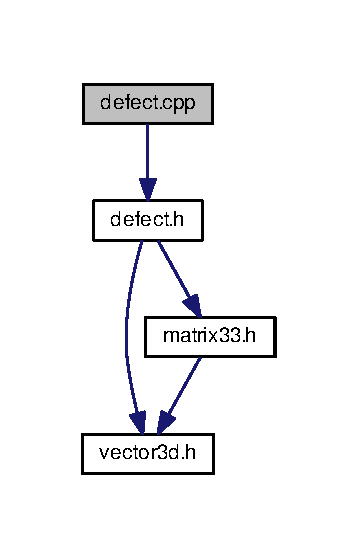
\includegraphics[width=200pt]{dd/dcf/defect_8cpp__incl}
\end{center}
\end{figure}


\subsection{\-Detailed \-Description}
\-Definition of member functions of the \hyperlink{classDefect}{\-Defect} class. \begin{DoxyAuthor}{\-Author}
\-Adhish \-Majumdar 
\end{DoxyAuthor}
\begin{DoxyVersion}{\-Version}
0.\-0 
\end{DoxyVersion}
\begin{DoxyDate}{\-Date}
22/04/2013
\end{DoxyDate}
\-This file defines the member functions of the \hyperlink{classDefect}{\-Defect} class representing a single defect in the simulation. 

\-Definition in file \hyperlink{defect_8cpp_source}{defect.\-cpp}.


\hypertarget{defect_8h}{\section{defect.\-h \-File \-Reference}
\label{df/d55/defect_8h}\index{defect.\-h@{defect.\-h}}
}


\-Definition of the \hyperlink{classDefect}{\-Defect} class.  


{\ttfamily \#include \char`\"{}vector3d.\-h\char`\"{}}\*
{\ttfamily \#include \char`\"{}matrix33.\-h\char`\"{}}\*
{\ttfamily \#include \char`\"{}stress.\-h\char`\"{}}\*
\-Include dependency graph for defect.\-h\-:\nopagebreak
\begin{figure}[H]
\begin{center}
\leavevmode
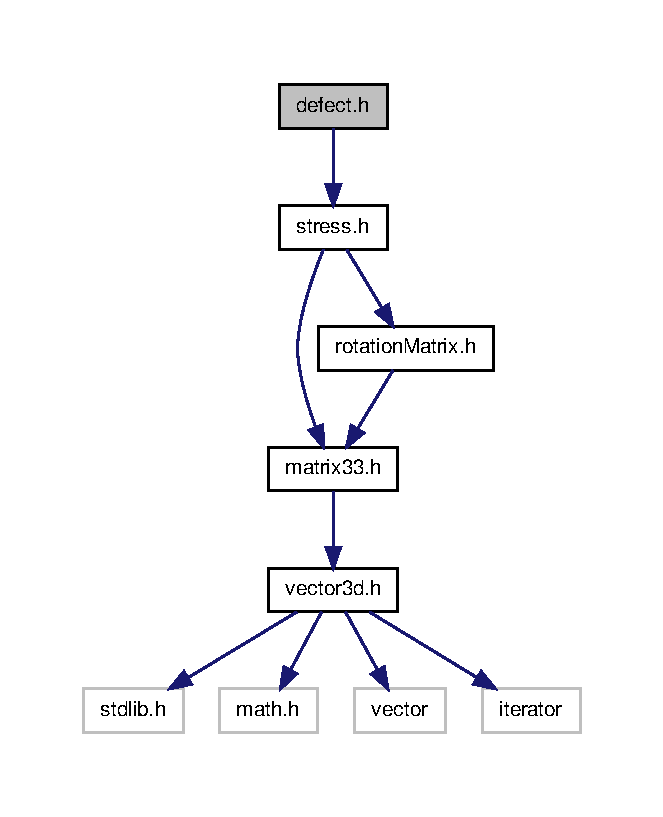
\includegraphics[width=256pt]{d2/d68/defect_8h__incl}
\end{center}
\end{figure}
\-This graph shows which files directly or indirectly include this file\-:\nopagebreak
\begin{figure}[H]
\begin{center}
\leavevmode
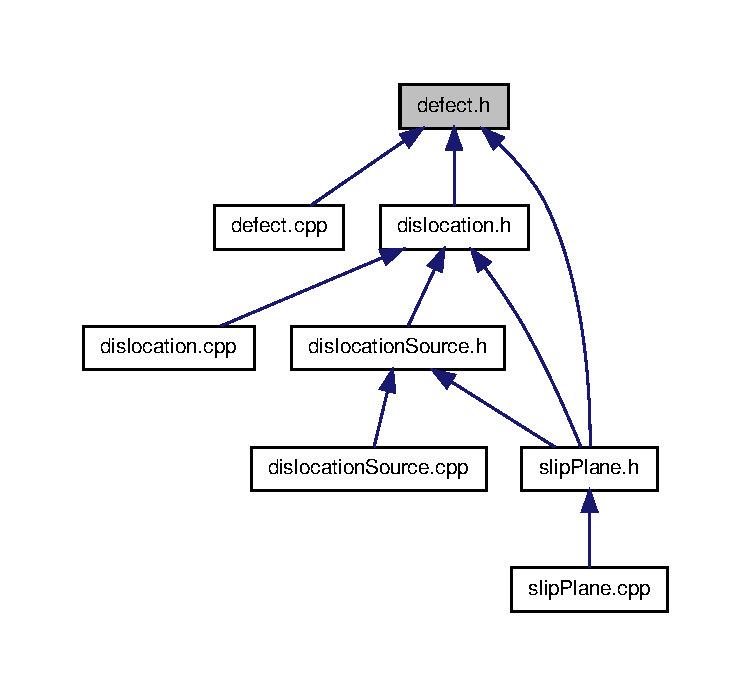
\includegraphics[width=230pt]{dc/d4d/defect_8h__dep__incl}
\end{center}
\end{figure}
\subsection*{\-Data \-Structures}
\begin{DoxyCompactItemize}
\item 
class \hyperlink{classDefect}{\-Defect}
\begin{DoxyCompactList}\small\item\em \-Class \hyperlink{classDefect}{\-Defect} representing a generic defect in a material. \end{DoxyCompactList}\end{DoxyCompactItemize}


\subsection{\-Detailed \-Description}
\-Definition of the \hyperlink{classDefect}{\-Defect} class. \begin{DoxyAuthor}{\-Author}
\-Adhish \-Majumdar 
\end{DoxyAuthor}
\begin{DoxyVersion}{\-Version}
0.\-0 
\end{DoxyVersion}
\begin{DoxyDate}{\-Date}
22/04/2013
\end{DoxyDate}
\-This file defines the \hyperlink{classDefect}{\-Defect} class representing an defect in the simulation. \-This is simply a generic description class with virtual functions. \-Later classes like dislocations, precipitates, boundaries etc will inherit from this class. 

\-Definition in file \hyperlink{defect_8h_source}{defect.\-h}.


\hypertarget{matrix33_8cpp}{\section{matrix33.\-cpp \-File \-Reference}
\label{d8/d8e/matrix33_8cpp}\index{matrix33.\-cpp@{matrix33.\-cpp}}
}


\-Definition of the member functions and operators of the \hyperlink{classMatrix33}{\-Matrix33} class.  


{\ttfamily \#include \char`\"{}matrix33.\-h\char`\"{}}\*
\-Include dependency graph for matrix33.\-cpp\-:\nopagebreak
\begin{figure}[H]
\begin{center}
\leavevmode
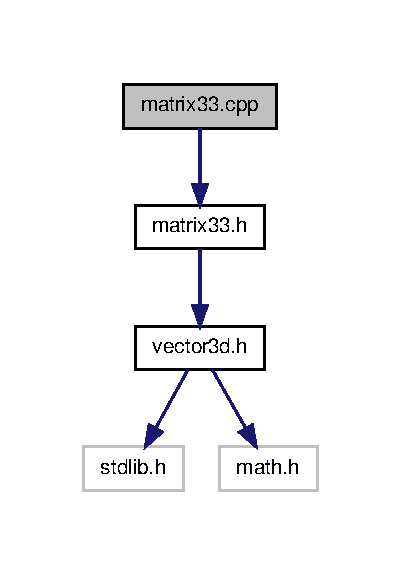
\includegraphics[width=318pt]{d8/d6d/matrix33_8cpp__incl}
\end{center}
\end{figure}


\subsection{\-Detailed \-Description}
\-Definition of the member functions and operators of the \hyperlink{classMatrix33}{\-Matrix33} class. \begin{DoxyAuthor}{\-Author}
\-Adhish \-Majumdar 
\end{DoxyAuthor}
\begin{DoxyVersion}{\-Version}
1.\-0 
\end{DoxyVersion}
\begin{DoxyDate}{\-Date}
04/06/2013
\end{DoxyDate}
\-This file defines the member functions and operators of the \hyperlink{classMatrix33}{\-Matrix33} class representing a 3x3 matrix in the simulation. 

\-Definition in file \hyperlink{matrix33_8cpp_source}{matrix33.\-cpp}.


\hypertarget{matrix33_8h}{\section{matrix33.\-h File Reference}
\label{db/d46/matrix33_8h}\index{matrix33.\-h@{matrix33.\-h}}
}


Definition of the \hyperlink{classMatrix33}{Matrix33} class.  


{\ttfamily \#include \char`\"{}vector3d.\-h\char`\"{}}\\*
Include dependency graph for matrix33.\-h\-:\nopagebreak
\begin{figure}[H]
\begin{center}
\leavevmode
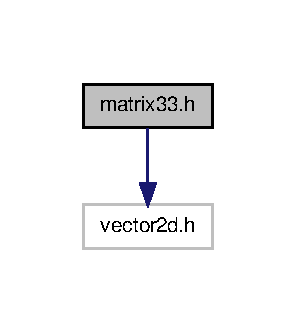
\includegraphics[width=142pt]{d7/dc7/matrix33_8h__incl}
\end{center}
\end{figure}
This graph shows which files directly or indirectly include this file\-:
\nopagebreak
\begin{figure}[H]
\begin{center}
\leavevmode
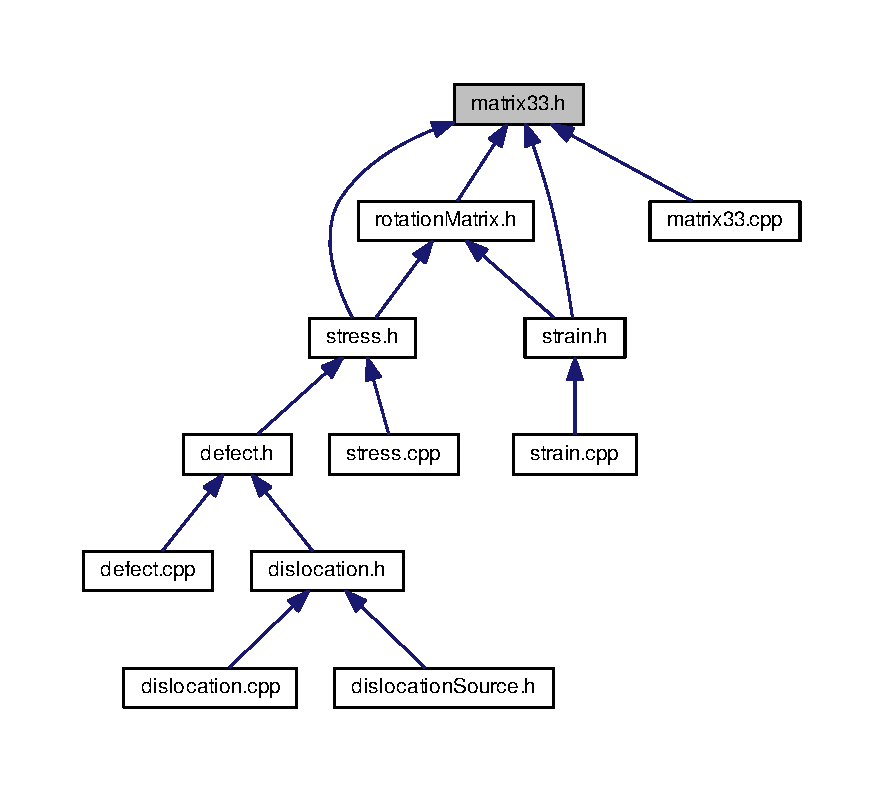
\includegraphics[width=301pt]{dd/d84/matrix33_8h__dep__incl}
\end{center}
\end{figure}
\subsection*{Data Structures}
\begin{DoxyCompactItemize}
\item 
class \hyperlink{classMatrix33}{Matrix33}
\begin{DoxyCompactList}\small\item\em \hyperlink{classMatrix33}{Matrix33} class representing a 3x3 square matrix. \end{DoxyCompactList}\end{DoxyCompactItemize}


\subsection{Detailed Description}
Definition of the \hyperlink{classMatrix33}{Matrix33} class. \begin{DoxyAuthor}{Author}
Adhish Majumdar 
\end{DoxyAuthor}
\begin{DoxyVersion}{Version}
0.\-0 
\end{DoxyVersion}
\begin{DoxyDate}{Date}
22/04/2013
\end{DoxyDate}
This file defines the \hyperlink{classMatrix33}{Matrix33} class representing a 3x3 matrix in the simulation. 

Definition in file \hyperlink{matrix33_8h_source}{matrix33.\-h}.


\hypertarget{stress_8cpp}{\section{stress.\-cpp \-File \-Reference}
\label{d4/d58/stress_8cpp}\index{stress.\-cpp@{stress.\-cpp}}
}


\-Definition of the member functions if the \hyperlink{classStress}{\-Stress} class.  


{\ttfamily \#include \char`\"{}stress.\-h\char`\"{}}\*
\-Include dependency graph for stress.\-cpp\-:
\nopagebreak
\begin{figure}[H]
\begin{center}
\leavevmode
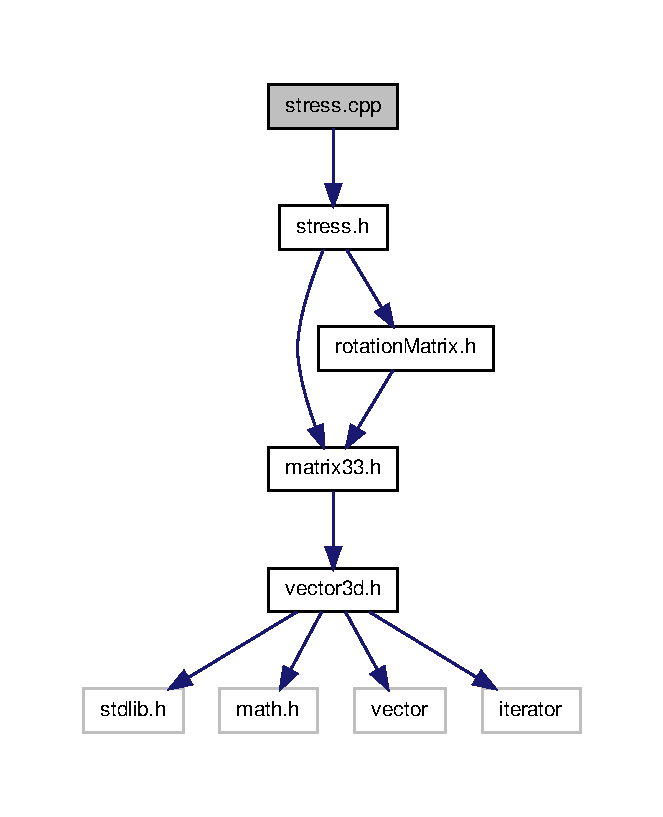
\includegraphics[width=188pt]{d0/d28/stress_8cpp__incl}
\end{center}
\end{figure}


\subsection{\-Detailed \-Description}
\-Definition of the member functions if the \hyperlink{classStress}{\-Stress} class. \begin{DoxyAuthor}{\-Author}
\-Adhish \-Majumdar 
\end{DoxyAuthor}
\begin{DoxyVersion}{\-Version}
0.\-0 
\end{DoxyVersion}
\begin{DoxyDate}{\-Date}
22/04/2013
\end{DoxyDate}
\-This file defines the member functions of the \hyperlink{classStress}{\-Stress} class for the stress tensor. 

\-Definition in file \hyperlink{stress_8cpp_source}{stress.\-cpp}.


\hypertarget{stress_8h}{\section{stress.\-h File Reference}
\label{d2/d50/stress_8h}\index{stress.\-h@{stress.\-h}}
}


Definition of the \hyperlink{classStress}{Stress} class.  


{\ttfamily \#include \char`\"{}matrix33.\-h\char`\"{}}\\*
{\ttfamily \#include \char`\"{}rotation\-Matrix.\-h\char`\"{}}\\*
Include dependency graph for stress.\-h\-:
\nopagebreak
\begin{figure}[H]
\begin{center}
\leavevmode
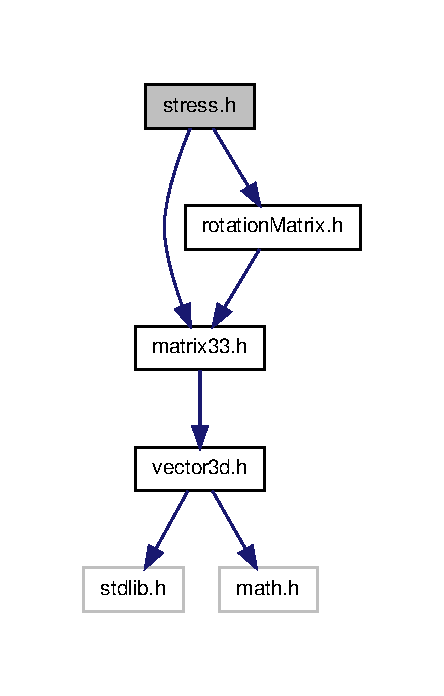
\includegraphics[width=213pt]{df/d2b/stress_8h__incl}
\end{center}
\end{figure}
This graph shows which files directly or indirectly include this file\-:
\nopagebreak
\begin{figure}[H]
\begin{center}
\leavevmode
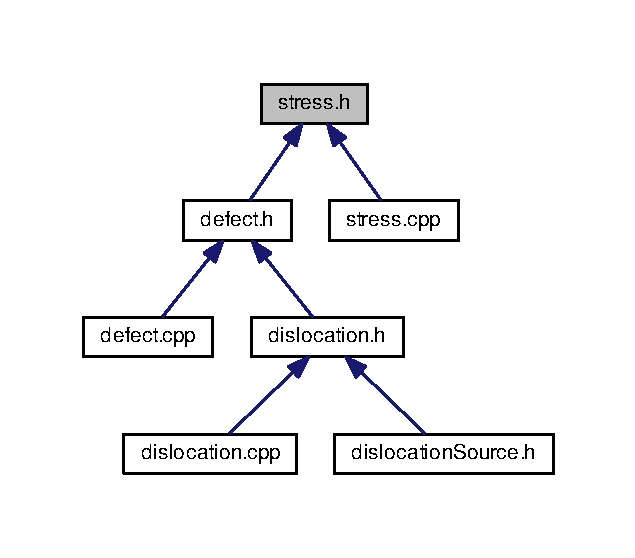
\includegraphics[width=350pt]{dc/d05/stress_8h__dep__incl}
\end{center}
\end{figure}
\subsection*{Data Structures}
\begin{DoxyCompactItemize}
\item 
class \hyperlink{classStress}{Stress}
\begin{DoxyCompactList}\small\item\em \hyperlink{classStress}{Stress} class to represent the stress tensor. \end{DoxyCompactList}\end{DoxyCompactItemize}


\subsection{Detailed Description}
Definition of the \hyperlink{classStress}{Stress} class. \begin{DoxyAuthor}{Author}
Adhish Majumdar 
\end{DoxyAuthor}
\begin{DoxyVersion}{Version}
1.\-0 
\end{DoxyVersion}
\begin{DoxyDate}{Date}
05/06/2013
\end{DoxyDate}
This file defines the \hyperlink{classStress}{Stress} class for the stress tensor. 

Definition in file \hyperlink{stress_8h_source}{stress.\-h}.


\hypertarget{vector3d_8cpp}{\section{vector3d.\-cpp File Reference}
\label{d7/d35/vector3d_8cpp}\index{vector3d.\-cpp@{vector3d.\-cpp}}
}


Definition of the \hyperlink{classVector3d}{Vector3d} class and its functions.  


{\ttfamily \#include \char`\"{}vector3d.\-h\char`\"{}}\\*
Include dependency graph for vector3d.\-cpp\-:\nopagebreak
\begin{figure}[H]
\begin{center}
\leavevmode
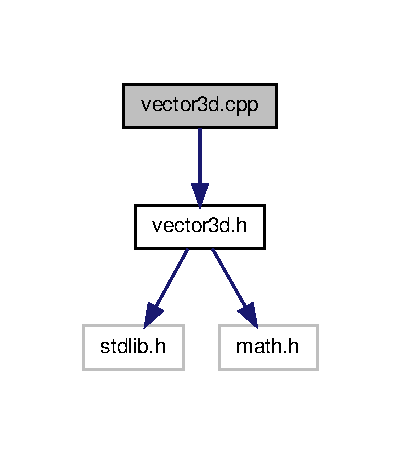
\includegraphics[width=154pt]{d5/d7b/vector3d_8cpp__incl}
\end{center}
\end{figure}


\subsection{Detailed Description}
Definition of the \hyperlink{classVector3d}{Vector3d} class and its functions. \begin{DoxyAuthor}{Author}
Adhish Majumdar 
\end{DoxyAuthor}
\begin{DoxyVersion}{Version}
0.\-0 
\end{DoxyVersion}
\begin{DoxyDate}{Date}
15/04/2013
\end{DoxyDate}
This file defines the \hyperlink{classVector3d}{Vector3d} class representing a single 3-\/dimensional vector in the simulation and its member functions and operators. 

Definition in file \hyperlink{vector3d_8cpp_source}{vector3d.\-cpp}.


\hypertarget{vector3d_8h}{\section{vector3d.\-h File Reference}
\label{d9/df8/vector3d_8h}\index{vector3d.\-h@{vector3d.\-h}}
}


Definition of the \hyperlink{classVector3d}{Vector3d} class.  


{\ttfamily \#include $<$stdlib.\-h$>$}\\*
{\ttfamily \#include $<$math.\-h$>$}\\*
{\ttfamily \#include $<$vector$>$}\\*
{\ttfamily \#include $<$iterator$>$}\\*
Include dependency graph for vector3d.\-h\-:
\nopagebreak
\begin{figure}[H]
\begin{center}
\leavevmode
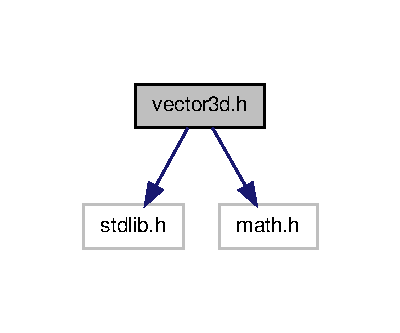
\includegraphics[width=318pt]{dc/db1/vector3d_8h__incl}
\end{center}
\end{figure}
This graph shows which files directly or indirectly include this file\-:
\nopagebreak
\begin{figure}[H]
\begin{center}
\leavevmode
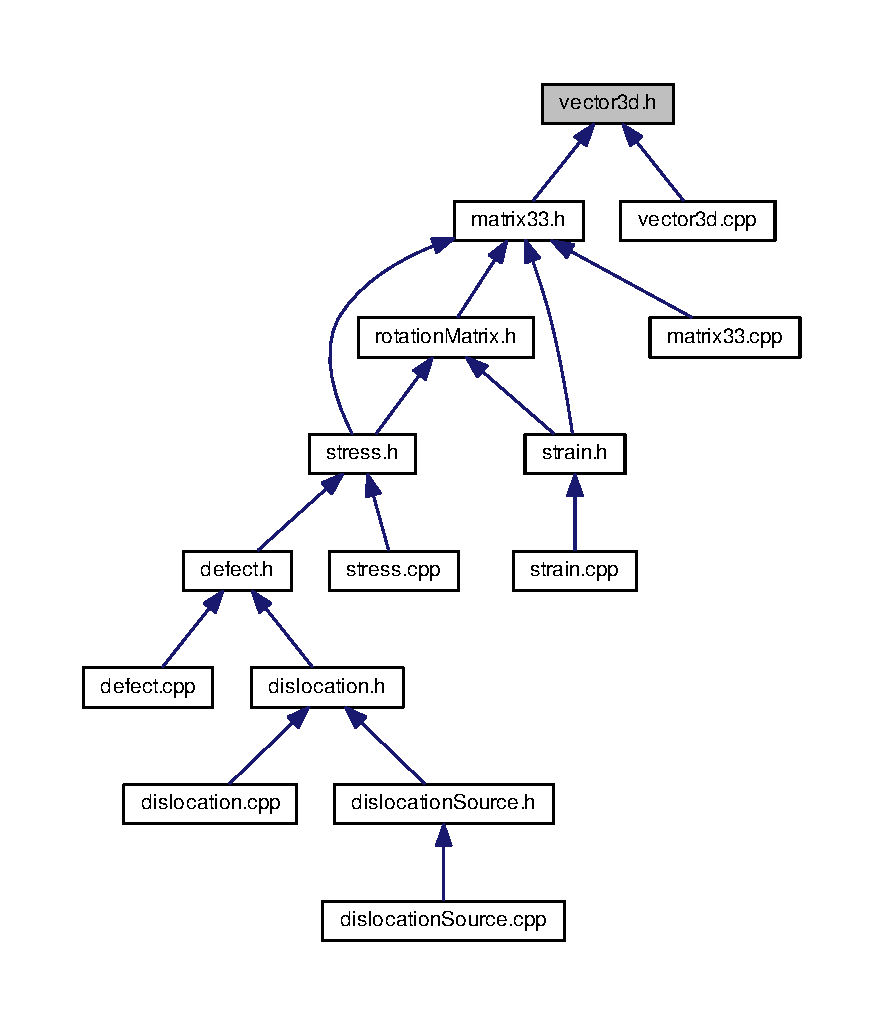
\includegraphics[width=350pt]{d3/dd7/vector3d_8h__dep__incl}
\end{center}
\end{figure}
\subsection*{Data Structures}
\begin{DoxyCompactItemize}
\item 
class \hyperlink{classVector3d}{Vector3d}
\begin{DoxyCompactList}\small\item\em \hyperlink{classVector3d}{Vector3d} class representing a single 3-\/dimensional vector in the simulation. \end{DoxyCompactList}\end{DoxyCompactItemize}


\subsection{Detailed Description}
Definition of the \hyperlink{classVector3d}{Vector3d} class. \begin{DoxyAuthor}{Author}
Adhish Majumdar 
\end{DoxyAuthor}
\begin{DoxyVersion}{Version}
1.\-0 
\end{DoxyVersion}
\begin{DoxyDate}{Date}
04/06/2013
\end{DoxyDate}
This file defines the \hyperlink{classVector3d}{Vector3d} class representing a single 3-\/dimensional vector in the simulation. 

Definition in file \hyperlink{vector3d_8h_source}{vector3d.\-h}.


\printindex
\end{document}
